
\documentclass[a4paper,12pt]{extarticle}
\usepackage{tempora}
\usepackage{geometry}
\usepackage[T1,T2A]{fontenc}
\usepackage[utf8]{inputenc}
\usepackage[english,russian]{babel}
\usepackage{amsmath}
\usepackage{amsthm}
\usepackage{amssymb}
\usepackage{fancyhdr}
\usepackage{setspace}
\usepackage{caption}
\usepackage{needspace}
\usepackage[normalem]{ulem}
\usepackage{graphicx}
\usepackage{float}
\usepackage{colortbl}
\usepackage{tikz}
\usepackage{pgf}
\usepackage{subcaption}
\ExplSyntaxOn
\cs_if_exist:NT \FirstAidNeededT
  {\cs_set:Npn \FirstAidNeededT #1#2#3 {\exp_args:Ncx\str_if_eq:onT{ver@#1.#2}{#3}}}
\ExplSyntaxOff
\usepackage{listings}
\usepackage{indentfirst}
\usepackage{csquotes}
\usepackage[
backend=biber,
style=numeric,
maxbibnames=99
]{biblatex}
\addbibresource{refs.bib}
\AtBeginBibliography{\raggedright\sloppy}
\usepackage[colorlinks,citecolor=blue,linkcolor=blue,bookmarks=false,hypertexnames=true,urlcolor=blue]{hyperref}
\usepackage{mathtools}
\usepackage{booktabs}
\usepackage[flushleft]{threeparttable}
\usepackage{tablefootnote}
\usepackage{chngcntr}


\graphicspath{{graphics/}}
\lstset{breaklines=true,basicstyle=\ttfamily\small}
\captionsetup{labelsep=endash}
\captionsetup[table]{justification=raggedright,singlelinecheck=false,position=top}
\DeclareCaptionLabelFormat{appendixfigure}{#2}
\DeclareCaptionLabelSeparator{appendixdash}{ - }
\addto\captionsrussian{\def\figurename{Рисунок}}
\addto\captionsrussian{\def\tablename{Таблица}}

\makeatletter
% \renewcommand{\@biblabel}[1]{#1.}
\makeatother

\geometry{left=2.5cm}
\geometry{right=1.0cm}
\geometry{top=2.0cm}
\geometry{bottom=2.0cm}
\setlength{\parindent}{1.25cm}
\renewcommand{\baselinestretch}{1.5}
\setlength{\emergencystretch}{3em}

\newcommand{\bibref}[3]{\hyperlink{#1}{#2 (#3)}}
\newcommand{\sourcecite}[1]{\hyperref[#1]{[\ref*{#1}]}}
\addto\captionsrussian{\def\refname{Список использованных источников}}

\renewcommand{\theenumi}{\arabic{enumi}}
\renewcommand{\labelenumi}{\arabic{enumi}}
\renewcommand{\theenumii}{.\arabic{enumii}}
\renewcommand{\labelenumii}{\arabic{enumi}.\arabic{enumii}.}
\renewcommand{\theenumiii}{.\arabic{enumiii}}
\renewcommand{\labelenumiii}{\arabic{enumi}.\arabic{enumii}.\arabic{enumiii}.}

\providecommand{\chapter}[1]{\section{#1}}
\providecommand{\chapter*}[1]{\section*{#1}}

\makeatletter
\renewcommand\section{\@startsection{section}{1}{\z@}%
  {-3.5ex \@plus -1ex \@minus -.2ex}%
  {2.3ex \@plus.2ex}%
  {\normalfont\Large\bfseries\Needspace{8\baselineskip}}}
\renewcommand\subsection{\@startsection{subsection}{2}{\z@}%
  {-3.25ex\@plus -1ex \@minus -.2ex}%
  {1.5ex \@plus .2ex}%
  {\normalfont\large\bfseries\Needspace{6\baselineskip}}}
\renewcommand\subsubsection{\@startsection{subsubsection}{3}{\z@}%
  {-3.25ex\@plus -1ex \@minus -.2ex}%
  {1.5ex \@plus .2ex}%
  {\normalfont\normalsize\bfseries\Needspace{5\baselineskip}}}
\makeatother

\pagestyle{fancy}
\fancyhf{}
\fancyfoot[C]{\thepage}
\renewcommand{\headrulewidth}{0pt}
\renewcommand{\footrulewidth}{0pt}


\begin{document}
\begin{titlepage}
\newpage
\thispagestyle{empty}
\setstretch{1.0}
\small

\begin{center}
\textbf{ФЕДЕРАЛЬНОЕ ГОСУДАРСТВЕННОЕ АВТОНОМНОЕ ОБРАЗОВАТЕЛЬНОЕ УЧРЕЖДЕНИЕ}\\
\textbf{ВЫСШЕГО ОБРАЗОВАНИЯ}\\
\textbf{``НАЦИОНАЛЬНЫЙ ИССЛЕДОВАТЕЛЬСКИЙ УНИВЕРСИТЕТ}\\
\textbf{``ВЫСШАЯ ШКОЛА ЭКОНОМИКИ''}\\
\textbf{ФАКУЛЬТЕТ КОМПЬЮТЕРНЫХ НАУК}
\end{center}

\vspace{2.4cm}

\begin{center}
\uline{Вальсамакин Александр Александрович}\\
\uline{Удалов Даниил Григорьевич}
\end{center}

\vspace{1.4cm}

\begin{center}
МАГИСТЕРСКАЯ ДИССЕРТАЦИЯ
\end{center}

\vspace{0.6cm}

\begin{center}
\textbf{\uline{Улучшение генерации музыки с помощью обучения с подкреплением}}
\end{center}

\vspace{0.3cm}

\begin{center}
\textbf{\uline{Enhanced Music Generation via Reinforcement Learning}}
\end{center}

\vspace{0.6cm}

\begin{center}
по направлению подготовки \uline{01.04.02 Прикладная математика и информатика}\\
образовательная программа «Искусственный интеллект»
\end{center}

\vspace{1.8cm}

\noindent Студенты\\
\makebox[6cm]{\hrulefill}\\
А.А. Вальсамакин\\[0.35cm]
\makebox[6cm]{\hrulefill}\\
Д.Г. Удалов

\vspace{0.9cm}

\noindent Научный руководитель

\vspace{-0.2cm}

\begin{flushright}
к.ф.-м.н., доцент\\
\makebox[6cm]{\hrulefill}\\
Е.О. Кантонистова
\end{flushright}

\vspace{0.45cm}

\begin{flushright}
Соруководитель\\
Департамент больших данных и информационного поиска\\
\makebox[6cm]{\hrulefill}\\
П.М. Гринберг
\end{flushright}

\vspace{\fill}

\begin{center}
Москва 2026
\end{center}

\end{titlepage}
\newpage
\setcounter{page}{2}
\thispagestyle{empty}

{
    \hypersetup{linkcolor=black}
    \tableofcontents
}

\newpage


\section*{Аннотация}
\addcontentsline{toc}{section}{Аннотация}

В работе рассматривается задача улучшения генерации MIDI-фрагментов по текстовому описанию. Базовая text-to-MIDI модель способна порождать синтаксически корректные музыкальные последовательности, однако стандартное контролируемое обучение не задаёт напрямую критерии качества готового фрагмента: тональную согласованность, устойчивость ритма, осмысленную плотность нот, соотношение мелодии и аккомпанемента, а также соответствие музыкального результата текстовому запросу.

Для решения этой проблемы исследуется схема последующего дообучения модели с использованием GRPO. Для одного текстового запроса генерируется группа MIDI-кандидатов, после чего они оцениваются не по отдельным токенам, а как завершённые музыкальные фрагменты. В качестве обучающего сигнала используются две группы наград: правила, основанные на музыкально-теоретических и статистических признаках, и оценка внешнего графового критика. Правила учитывают тональность, ритмическую структуру, плотность нот, долю ударных событий и другие свойства MIDI. Графовый критик строится отдельно: музыкальный фрагмент преобразуется в гетерогенный граф, в котором вершины соответствуют нотам, аккордам, тактам и временным позициям, а рёбра отражают временные и структурные связи. Для обучения критика используется корпус HookTheory Dataset, содержащий разметку мелодии, гармонии, тональности и метрической структуры. Рассматривается схема из графового учителя и графового ученика: учитель обучается различать корректные и искажённые музыкальные графы, а ученик приближает его оценку по признакам, извлекаемым из MIDI.

Экспериментальная часть включает несколько режимов дообучения: обучение по правилам, обучение по графовому критику, а также комбинированный сценарий, в котором критик применяется после предварительного rule-based этапа. Качество моделей анализируется по внутренним наградам, A/B-сравнениям с базовой моделью и внешней оценке языковой модели, работающей с ABC-представлением MIDI. Полученные результаты показывают, что последующее дообучение может смещать распределение генераций в сторону более предпочтительных по заданному критерию фрагментов, однако эффект зависит от качества награды, выбора запросов и устойчивости самого критика.

\textbf{Ключевые слова:} text-to-MIDI, символическая музыка, большие языковые модели, обучение с подкреплением, GRPO, графовые нейронные сети.

\newpage


\section*{Введение}
\addcontentsline{toc}{section}{Введение}

Генерация музыки по текстовому описанию находится на пересечении обработки естественного языка, символьной музыкальной генерации и задач управляемой музыкальной генерации. В такой постановке модель должна не просто сгенерировать правдоподобную последовательность нот, но и согласовать музыкальный результат с текстовым запросом: жанром, настроением, фактурой, инструментальным составом и структурой~\sourcecite{ref:ji2023symbolic}, \sourcecite{ref:duan2025recent}, \sourcecite{ref:bhandari2025text2midi}. Именно поэтому задача \textit{text-to-MIDI} существенно сложнее обычной безусловной генерации: здесь нужно одновременно моделировать музыкальную последовательность и межмодальное соответствие текста и музыки.

Актуальность темы определяется двумя обстоятельствами. Во-первых, крупные языковые модели сделали реалистичным перенос методов дообучения по инструкциям и оптимизации по предпочтениям в музыкальную область~\sourcecite{ref:chatmusician}, \sourcecite{ref:mupt}, \sourcecite{ref:kumar2026far}. Во-вторых, даже сильные генераторы символьной музыки всё ещё слабо гарантируют гармоническую согласованность, развитие материала и устойчивую многодорожечную структуру~\sourcecite{ref:briot2017deep}, \sourcecite{ref:ji2020comprehensive}, \sourcecite{ref:duan2025recent}, \sourcecite{ref:lerch2025-eval}. Поэтому естественным направлением является дообучение модели по внешним критериям качества, а не только по цели максимизации вероятности обучающих последовательностей.

Цель работы состоит в исследовании возможности улучшить генерацию \textit{MIDI} по текстовому описанию с помощью обучения с подкреплением (\textit{RL}). Для этого необходимо: кратко описать релевантные формы представления музыкальных данных; выделить сильные и слабые стороны современных генеративных архитектур; рассмотреть существующие решения для генерации \textit{MIDI} по тексту; проанализировать метрики; и обосновать собственную схему дообучения, сочетающую \textit{Text2midi}, \textit{Group Relative Policy Optimization} (\textit
{GRPO}) и структурный графовый критик.

За выбор набора обучающих данных и обучение графового критика ответственен А. А. Вальсамакин

За дообучение text2midi модели и внедрение критика ответственен Д. Г. Удалов

\section*{Обзор литературы}
\addcontentsline{toc}{section}{Обзор литературы}

\subsection*{Символьное представление музыки}
\addcontentsline{toc}{subsection}{Символьное представление музыки}

Для задач композиционного моделирования наиболее естественным остаётся символьное представление, поскольку оно явно кодирует ноты, длительности, метрические позиции, темп, аккорды и структуру партий, то есть именно те сущности, которые важны при анализе гармонии и формы~\sourcecite{ref:briot2017deep}, \sourcecite{ref:ji2020comprehensive}, \sourcecite{ref:ji2023symbolic}. В отличие от звукового сигнала, символьные данные меньше зависят от тембра и студийной обработки и лучше подходят для композиционного контроля. Среди символьных форматов используются фортепианная матрица, ABC-нотация, \textit{MIDI} и его расширения; для практических генеративных систем именно \textit{MIDI} остаётся наиболее универсальным представлением благодаря стандартизованному событийно-временному формату и поддержке многодорожечности~\sourcecite{ref:ji2020comprehensive}, \sourcecite{ref:ji2023symbolic}, \sourcecite{ref:duan2025recent}.

Для генерации \textit{MIDI} по текстовому описанию это особенно важно. Если ABC-нотация удобна для применения языковых моделей как к обычному тексту, то \textit{MIDI} ближе к прикладной задаче: он допускает несколько инструментов, пригоден для воспроизведения, анализа и последующего редактирования. Поэтому обзор работ на ABC-нотации важен как обзор возможных методов адаптации крупных языковых моделей, но прикладная цель работы остаётся связанной именно с генерацией \textit{MIDI}-последовательностей~\sourcecite{ref:chatmusician}, \sourcecite{ref:wu2022texttomusic}, \sourcecite{ref:bhandari2025text2midi}.

\subsection*{Основные архитектуры генерации символьной музыки и их ограничения}
\addcontentsline{toc}{subsection}{Основные архитектуры генерации символьной музыки и их ограничения}

Современная музыкальная генерация опирается прежде всего на трансформеры, вариационные автокодировщики, генеративно-состязательные сети, диффузионные модели и крупные предварительно обученные языковые модели~\sourcecite{ref:ji2020comprehensive}, \sourcecite{ref:ji2023symbolic}, \sourcecite{ref:duan2025recent}. Трансформеры сегодня являются наиболее универсальным инструментом для последовательной генерации: они хорошо моделируют дальние зависимости и естественно применяются к событийным представлениям музыки, что показано, например, в \textit{Music Transformer}, \textit{Pop Music Transformer} и последующих работах~\sourcecite{ref:huang2018-music-transformer}, \sourcecite{ref:huangyang2020-remi}, \sourcecite{ref:hsiao2021-compound}. Их главный недостаток для генерации \textit{MIDI} по тексту --- высокая чувствительность к токенизации и отсутствие явной гарантии музыкально-теоретической согласованности.

Вариационные автокодировщики удобны для интерполяции и управления скрытым представлением, однако нередко уступают авторегрессионным моделям по локальной детализации и долгосрочной форме~\sourcecite{ref:roberts2018-musicvae}, \sourcecite{ref:duan2025recent}. Генеративно-состязательные сети сыграли заметную роль в многодорожечной генерации, но для дискретной символьной музыки остаются нестабильными и плохо согласуют глобальные музыкальные ограничения~\sourcecite{ref:dong2018-musegan}, \sourcecite{ref:duan2025recent}. Диффузионные модели показывают высокое качество и позволяют добавлять управление правилами, но обладают большой вычислительной стоимостью и пока не снимают проблему целостной формы~\sourcecite{ref:mittal2021-diffusion}, \sourcecite{ref:plasser2023-schmubert}, \sourcecite{ref:huang2024-ruleguided}, \sourcecite{ref:duan2025recent}. Наконец, подходы на основе крупных языковых моделей привлекательны возможностью совместной работы с текстом и музыкой, но они переносят в музыкальную область и типичные проблемы моделей, дообученных по инструкциям: потерю предметной точности при слабой адаптации и деградацию общих способностей при слишком агрессивном дообучении~\sourcecite{ref:chatmusician}, \sourcecite{ref:zeng2021-musicbert}, \sourcecite{ref:mupt}, \sourcecite{ref:kumar2026far}.

Таким образом, общий вывод обзора состоит в том, что ни одна архитектура сама по себе не обеспечивает одновременно хорошее текстово-музыкальное соответствие, теоретическую осмысленность и устойчивую структуру на длинных промежутках. Это и мотивирует переход к внешним критериям качества и подходам обучения с подкреплением~\sourcecite{ref:duan2025recent}, \sourcecite{ref:lerch2025-eval}.

\subsection*{Метрики и современные решения генерации \textit{MIDI} по тексту}
\addcontentsline{toc}{subsection}{Метрики и современные решения генерации \textit{MIDI} по тексту}

Оценка генеративных музыкальных систем остаётся отдельной сложной задачей. Субъективные экспертные оценки хорошо отражают музыкальность результата, но плохо масштабируются. Объективные статистические метрики позволяют сравнивать распределения событий, однако часто слабо коррелируют с музыкальной выразительностью. Метрики на основе вложений и косвенные показатели для конкретной задачи частично закрывают этот разрыв, но не устраняют его полностью~\sourcecite{ref:yang-lerch2019-eval}, \sourcecite{ref:lerch2025-eval}, \sourcecite{ref:retkowski2024-fmd}, \sourcecite{ref:wu2025-clamp2}. Для генерации \textit{MIDI} по тексту этого недостаточно вдвойне: необходимо оценивать и внутреннюю музыкальную правдоподобность, и согласование с текстом.

Содержательный переход к условной символьной генерации по тексту произошёл от работ по управлению эмоциями и атрибутами к системам, где текст напрямую связан с музыкальным выводом~\sourcecite{ref:zhang2020-butter}, \sourcecite{ref:lu2023-musecoco}. Одним из наиболее прикладных решений стала модель \textit{Text2midi}, формулирующая задачу как генерацию символьной музыки по текстовым описаниям~\sourcecite{ref:bhandari2025text2midi}. В соседнем направлении \textit{ChatMusician} трактует музыку как второй язык и показывает, что крупные языковые модели можно адаптировать для музыкального понимания и генерации~\sourcecite{ref:chatmusician}. Однако такие подходы по-разному балансируют между удобством текстового интерфейса и музыкальной строгостью: ABC-нотация облегчает перенос методов обработки естественного языка, но не совпадает с прикладной целью генерации \textit{MIDI}; сквозная генерация \textit{MIDI} по тексту ближе к практике, но сильнее зависит от качества текстовых подписей и сложности многодорожечных примеров~\sourcecite{ref:wu2022texttomusic}, \sourcecite{ref:bhandari2025text2midi}.

Особенно важной для данной работы является статья \textit{How Far Can Pretrained LLMs Go in Symbolic Music? Controlled Comparisons of Supervised and Preference-based Adaptation}~\sourcecite{ref:kumar2026far}. Авторы сравнивают LLaMA 3.1 8B, дообученную по инструкциям, контролируемое дообучение (\textit{SFT}), прямую оптимизацию предпочтений (\textit{DPO}) и специализированную музыкальную базовую модель на задачах генерации и понимания в ABC-нотации. Вариант обучения по предпочтениям строится не на явном критике, а на слабых предпочтениях: ``отвергнутые'' ответы получают путём музыкально мотивированных деградаций целевой ABC-записи при сохранении синтаксической корректности; после этого применяется \textit{DPO}. Результаты работы показывают, что \textit{SFT} обычно лучше адаптирует модель к музыкальному домену по метрикам на уровне токенов, тогда как \textit{DPO} в большей степени сохраняет общие возможности модели, но не даёт устойчивого преимущества в музыкальном качестве. Авторы также специально подчёркивают, что перплексия и \textit{Fréchet Music Distance} ведут себя по-разному и не дают единой картины качества~\sourcecite{ref:kumar2026far}. Для настоящей работы эта статья важна в двух отношениях: она подтверждает полезность адаптации по предпочтениям в символьной музыке, но одновременно показывает, что слабого сигнала предпочтения недостаточно для уверенного улучшения структурного качества. Следовательно, вместо неявного сигнала предпочтения целесообразно рассмотреть более предметно ориентированный внешний критик.

\subsection*{Предлагаемый подход}
\addcontentsline{toc}{subsection}{Предлагаемый подход}

В качестве базовой системы в работе рассматривается \textit{Text2midi} как генератор \textit{MIDI} по текстовому описанию~\sourcecite{ref:bhandari2025text2midi}. Поверх него предлагается последующее дообучение с помощью \textit{Group Relative Policy Optimization} (\textit{GRPO}), где политика получает награду за соответствие музыки текстовому запросу. Такой базовый вариант близок к современным подходам согласования модели с целевыми критериями: модель оптимизируется не только по вероятности обучающих последовательностей, но и по внешнему критерию, отражающему конечную задачу~\sourcecite{ref:deepseekmath2024}, \sourcecite{ref:text2midi-inferalign}.

Основная идея расширения состоит в добавлении графового критика. Последовательность \textit{MIDI} преобразуется в музыкальный граф, в котором вершины и рёбра кодируют ноты, аккорды, моменты начала звучания, метрические позиции и связи между ними. Графовая нейронная сеть оценивает не токеновую правдоподобность, а структурные свойства результата: согласованность мелодии и гармонии, локальную функциональность аккордов, связь между событиями разных дорожек и более общую композиционную связность~\sourcecite{ref:karystinaios2023-chordgnn}, \sourcecite{ref:karystinaios2022-cadencegnn}, \sourcecite{ref:chen2018-harmony-mtl}, \sourcecite{ref:augmentednet}. Тогда итоговая награда сочетает как минимум два компонента: межмодальное согласование с текстом и структурную оценку графового критика.

Такой подход отличается и от чистого контролируемого дообучения (\textit{SFT}), и от обучения по предпочтениям на деградированных примерах. При \textit{SFT} модель приближает эмпирическое распределение токенов; при \textit{DPO} по слабым предпочтениям она учится предпочитать один выход другому. В предлагаемой схеме вводится предметно-информированный источник сигнала, напрямую ориентированный на музыкальную структуру.

\chapter{Данные и их предварительная обработка}

В данной главе описывается используемый набор данных, обосновывается выбор корпуса \textit{HookTheory Dataset}~\sourcecite{ref:hooktheory}, а также приводится процедура его предварительной обработки и преобразования в графовое представление. Отдельно рассматриваются основные статистические свойства корпуса, поскольку распределение музыкально-теоретических признаков напрямую влияет на качество обучения графового критика.

\subsection{Выбор набора данных}

В качестве основного источника данных в работе был выбран \textit{HookTheory Dataset}, компактная выгрузка данных из сервиса \textit{HookTheory}, данный сервис предоставляет пользователям возможность аннотации музыкальных произведений с точки зрения голосоведения и аккомпанемента (см. Рисунок~\ref{fig:hooktheory-example}).

\begin{figure}[htbp]
\centering
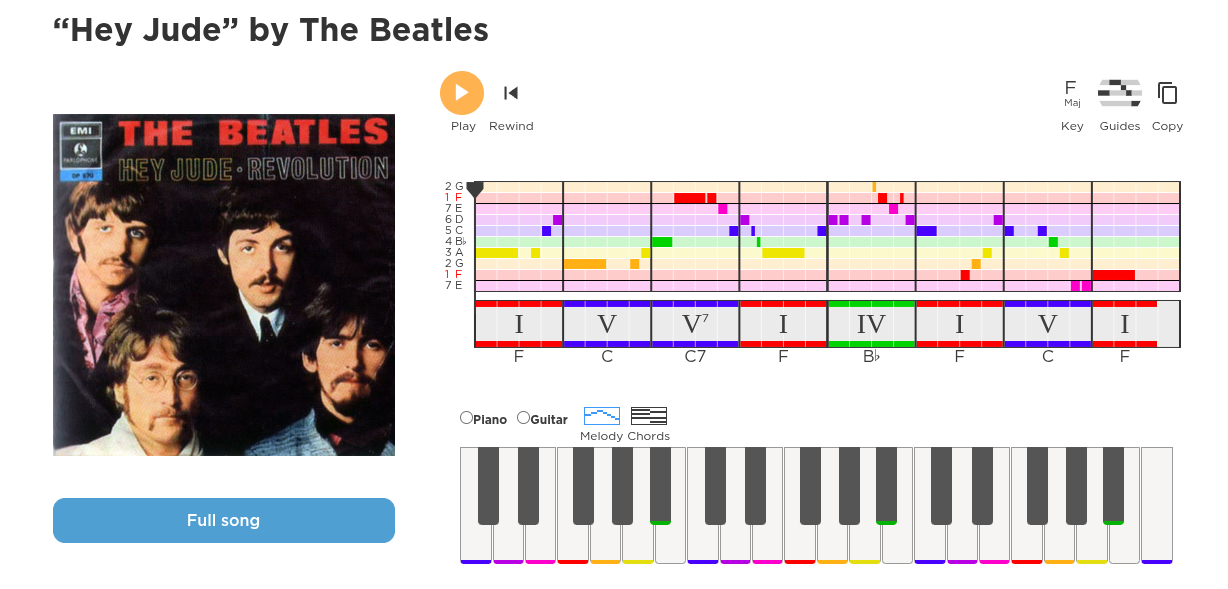
\includegraphics[width=0.94\textwidth,height=0.50\textheight,keepaspectratio]{HookTheory.png}
\caption{Пример песни и её аннотации с сайта \textit{HookTheory}}
\label{fig:hooktheory-example}
\end{figure}

Данный корпус содержит музыкальные фрагменты в символьном представлении, включающие аннотированные партии мелодии и гармонического сопровождения. Такой формат особенно важен для данной работы, поскольку целевая задача состоит в оценке и последующем улучшении музыкально-теоретической согласованности \textit{MIDI}-фрагментов, сгенерированных моделями генерации музыки по тексту.

В отличие от задачи генерации музыки напрямую, в данной работе требуется построить модель, способную анализировать уже имеющийся музыкальный фрагмент. Следовательно, существенным является не только наличие нотных событий, но и наличие информации о связи между мелодией, аккордами, тональностью, ладом и метрическим положением событий. \textit{HookTheory Dataset} близок к \textit{lead-sheet}-представлению музыкального материала: фрагмент описывается через мелодическую линию, аккордовую последовательность и связанную с ними музыкально-теоретическую разметку.

Такое представление позволяет строить обучающие примеры, в которых можно анализировать согласованность мелодии с текущим аккордом, соответствие аккордовой последовательности тональному контексту, появление неаккордовых звуков, связь музыкальных событий с метрической сеткой, а также локальные и глобальные нарушения музыкально-теоретической структуры.

Существуют более крупные \textit{MIDI}-корпуса, например \textit{Lakh MIDI Dataset}~\sourcecite{ref:lakh} и \textit{GiantMIDI-Piano}~\sourcecite{ref:giant-midi}. Они полезны для крупномасштабного предобучения моделей музыки в символьном представлении, однако не содержат достаточно подробной музыкально-теоретической разметки. В частности, в них отсутствует явная локальная связь между мелодическими событиями, аккордами, тональностью и гармонической функцией. Их использование потребовало бы отдельного этапа автоматического извлечения аккордов и тональностей, что внесло бы дополнительный шум в обучающие данные.

Другую группу составляют корпуса функционально-гармонического анализа, такие как \textit{When in Rome}~\sourcecite{ref:when-in-rome}, \textit{AugmentedNet}~\sourcecite{ref:augmentednet} и \textit{Distant Listening Corpus}~\sourcecite{ref:distant-listening}. Эти корпуса содержат более строгую теоретическую разметку, однако в основном ориентированы на классическую нотную традицию и задачу гармонического анализа с римскими цифрами. В данной работе, напротив, требуется модель, применимая к \textit{MIDI}/\textit{lead-sheet}-представлению и к результатам генерации \textit{MIDI} по текстовому описанию, которые часто ближе к популярной песенной музыке, чем к академической классической партитуре.

Также существуют крупные корпуса аккордовых последовательностей, например \textit{ChoCo}~\sourcecite{ref:choco} и \textit{Chordonomicon}~\sourcecite{ref:chordonomicon}. Они могут быть полезны для моделирования гармонических прогрессий, однако не всегда содержат мелодические партии и не позволяют напрямую оценивать соответствие конкретных нот \textit{MIDI} гармоническому контексту. Для данной работы это является существенным ограничением, поскольку модель должна оценивать не только правдоподобие аккордовой последовательности, но и согласованность мелодии и аккомпанемента.

При этом \textit{HookTheory Dataset} также имеет ограничения. Во-первых, в нём представлены не полные произведения, а короткие фрагменты, соответствующие отдельным секциям музыкальной формы: куплетам, припевам, вступлениям и т.д. Во-вторых, значительная часть разметки имеет пользовательское происхождение, что может приводить к отдельным ошибкам или неоднозначностям. В-третьих, корпус не является универсальным представлением всей западной музыкальной теории и преимущественно отражает практику \textit{lead-sheet}-разметки популярной музыки.

Тем не менее для поставленной задачи эти ограничения не являются критическими. Цель работы состоит не в построении универсальной системы академического гармонического анализа, а в обучении модели, способной оценивать музыкально-теоретическую согласованность \textit{MIDI}-фрагментов. В этом контексте \textit{HookTheory Dataset} представляет собой наиболее релевантный компромисс: он содержит достаточно богатую теоретическую информацию, включает связь между мелодией и гармонией и остаётся близким к формату \textit{MIDI}/\textit{lead-sheet}, характерному для современных задач генерации музыки в символьном представлении.

\subsection{Первичная обработка данных}

Исходный корпус \textit{HookTheory Dataset} хранится в формате \textit{JSON}. Каждый музыкальный фрагмент представлен отдельным \textit{JSON}-объектом, содержащим метаинформацию о треке, а также массивы мелодических и аккордовых событий. Поскольку не все поля исходного корпуса являются полезными для решаемой задачи, а часть признаков требует нормализации, обработка данных выполнялась в несколько этапов.

Общий процесс обработки включает: отбор информативных полей; нормализацию категориальных и числовых признаков; музыкально-теоретическую нормализацию тональностей, ладов, ступеней и аккордовых признаков; добавление специальных служебных полей; преобразование обработанных объектов в иерархические гетерогенные графы.

На первом этапе из исходного корпуса удаляются системные поля, не несущие музыкально-теоретической информации: ссылки на страницы песен в сервисе \textit{HookTheory}, информация об авторах и аннотаторах, служебные идентификаторы и другие поля, не используемые в модели. После этого для каждого музыкального фрагмента сохраняются общая метаинформация, массив мелодических событий, массив аккордовых событий и информация о секции музыкальной формы, если она представлена в данных.

Далее выполняется нормализация признаков. Тональности переводятся в частотные классы, то есть классы высот по модулю 12:

\[
\mathrm{C}/\mathrm{B}^{\sharp}\to 0,\quad
\mathrm{C}^{\sharp}/\mathrm{D}^{\flat}\to 1,\quad
\mathrm{D}\to 2,\quad \ldots,\quad
\mathrm{B}/\mathrm{C}^{\flat}\to 11.
\]

Аналогичные словари используются для ладов, мелодических ступеней, типов аккордов, ступеней аккордов, обращений и дополнительных аккордовых признаков. Такое представление позволяет заменить строковые категории числовыми идентификаторами и унифицировать дальнейшую обработку данных.

Отдельная нормализация применяется к ладам. Каждый лад представляется как упорядоченный массив смещений частотных классов относительно тоники:

\[
\small
\begin{alignedat}{2}
\mathrm{major} &= (0,2,4,5,7,9,11),\quad & \mathrm{minor} &= (0,2,3,5,7,8,10),\\
\mathrm{dorian} &= (0,2,3,5,7,9,10),\quad & \mathrm{phrygian} &= (0,1,3,5,7,8,10),\\
\mathrm{lydian} &= (0,2,4,6,7,9,11),\quad & \mathrm{mixolydian} &= (0,2,4,5,7,9,10),\\
\mathrm{locrian} &= (0,1,3,5,6,8,10). &
\end{alignedat}
\]

Такой формат описывает лад как набор относительных ступеней, то есть как смещения в полутонах от тоники по модулю 12. Абсолютные частотные классы для конкретной тональности вычисляются по формуле:
\[
pc_{\mathrm{abs}}=(pc_{\mathrm{tonic}}+pc_{\mathrm{mode}})\bmod 12,
\]

где $pc_{\mathrm{tonic}}$ --- частотный класс тоники, а $pc_{\mathrm{mode}}$ --- смещение внутри ладового шаблона.

Например, для тональности \textit{D major} имеем $pc_{\mathrm{tonic}}=2$. Тогда мажорный шаблон $(0,2,4,5,7,9,11)$ переходит в абсолютные частотные классы $(2,4,6,7,9,11,1)$.
Такое представление удобно тем, что один и тот же ладовый шаблон может использоваться для любой тональности. Кроме того, оно позволяет выполнять музыкально-теоретические операции: проверять принадлежность ноты ладу, определять нетональные ноты, сравнивать основной лад и заимствованные, строить аккорды по терциям и формировать кандидаты для аккордового оценщика.
После нормализации в словари категориальных признаков добавляются служебные поля: \textit{PAD}, \textit{MASK}, \textit{UNK}, \textit{NONE}. Они используются для параллельной обработки, маскирования признаков, обработки неизвестных значений и представления отсутствующих признаков.

На финальном этапе каждый музыкальный фрагмент преобразуется в иерархический гетерогенный граф. В графе используются следующие типы узлов: \textit{song}, \textit{bar}, \textit{onset}, \textit{note}, \textit{chord}.
Узел \textit{song} соответствует всему музыкальному фрагменту и содержит глобальные признаки: тональность, лад, размер, \textit{BPM} и длину фрагмента. Узел \textit{bar} задаёт такт внутри метрической сетки. Узел \textit{onset} соответствует временной позиции, в которой может начинаться одно или несколько событий. Узлы \textit{note} и \textit{chord} соответствуют мелодическим и аккордовым событиям.
Между узлами строятся иерархические и последовательные рёбра:

\[
\mathrm{song}\to\mathrm{bar}\to\mathrm{onset}\to\{\mathrm{note},\mathrm{chord}\},
\begin{aligned}
\mathrm{bar} &\to \mathrm{next\_bar},\\
\mathrm{onset} &\to \mathrm{next\_onset},\\
\mathrm{note} &\to \mathrm{next\_note},\\
\mathrm{chord} &\to \mathrm{covers\_note},\\
\mathrm{chord} &\to \mathrm{next\_chord}.
\end{aligned}
\]
Таким образом, исходный \textit{JSON}-объект \textit{HookTheory} преобразуется в структурированный граф, пригодный для обучения гетерогенной графовой нейронной сети (см. Рисунок~\ref{fig:graph-representation-schema}, Рисунок~\ref{fig:graph-representation-score}). Такое представление позволяет анализировать не только отдельные ноты и аккорды, но и отношения между ними, что является принципиально важным для построения музыкально-теоретического критика.

\begin{figure}[htbp]
\centering
\renewcommand{\thesubfigure}{\asbuk{subfigure}}
\begin{subfigure}[t]{0.46\textwidth}
\centering
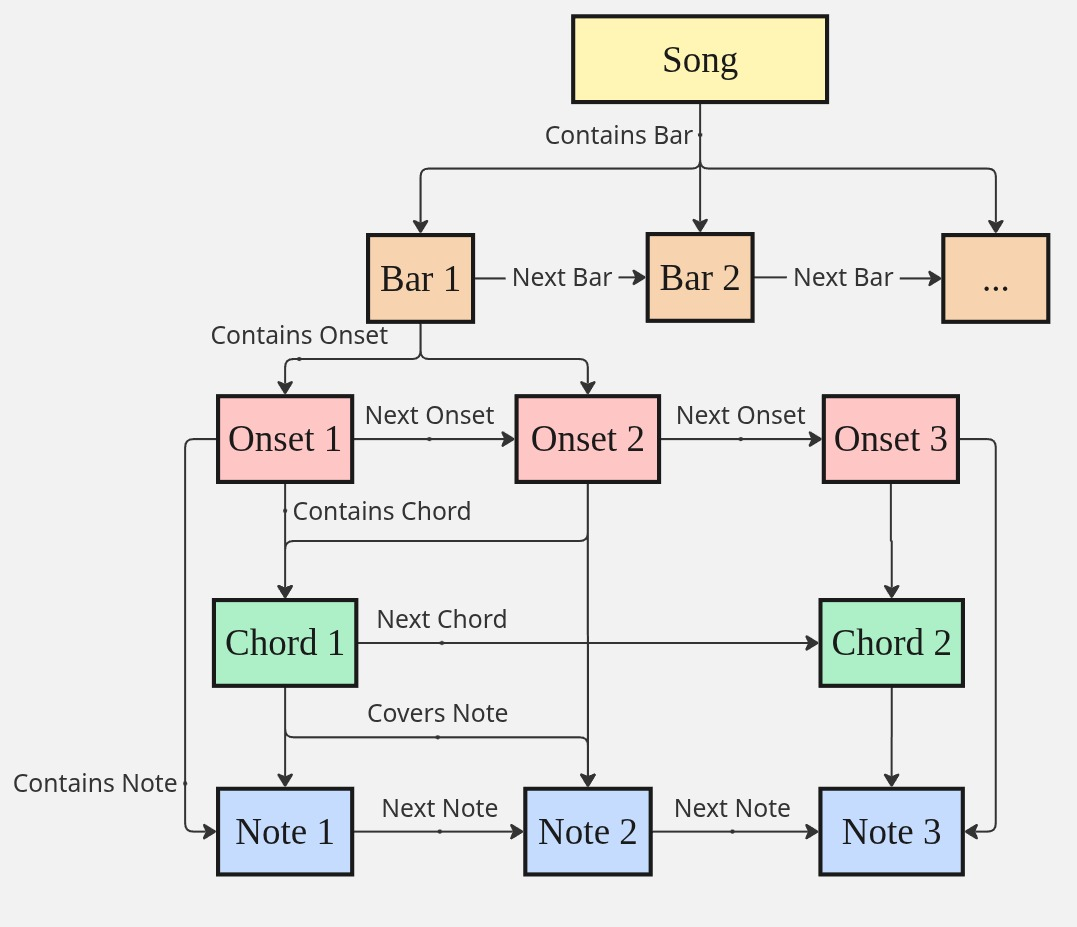
\includegraphics[width=\linewidth]{graph_hierarchy_edges.jpg}
\caption{Схема иерархии и типов связей}
\label{fig:graph-representation-schema}
\end{subfigure}\hfill
\begin{subfigure}[t]{0.46\textwidth}
\centering
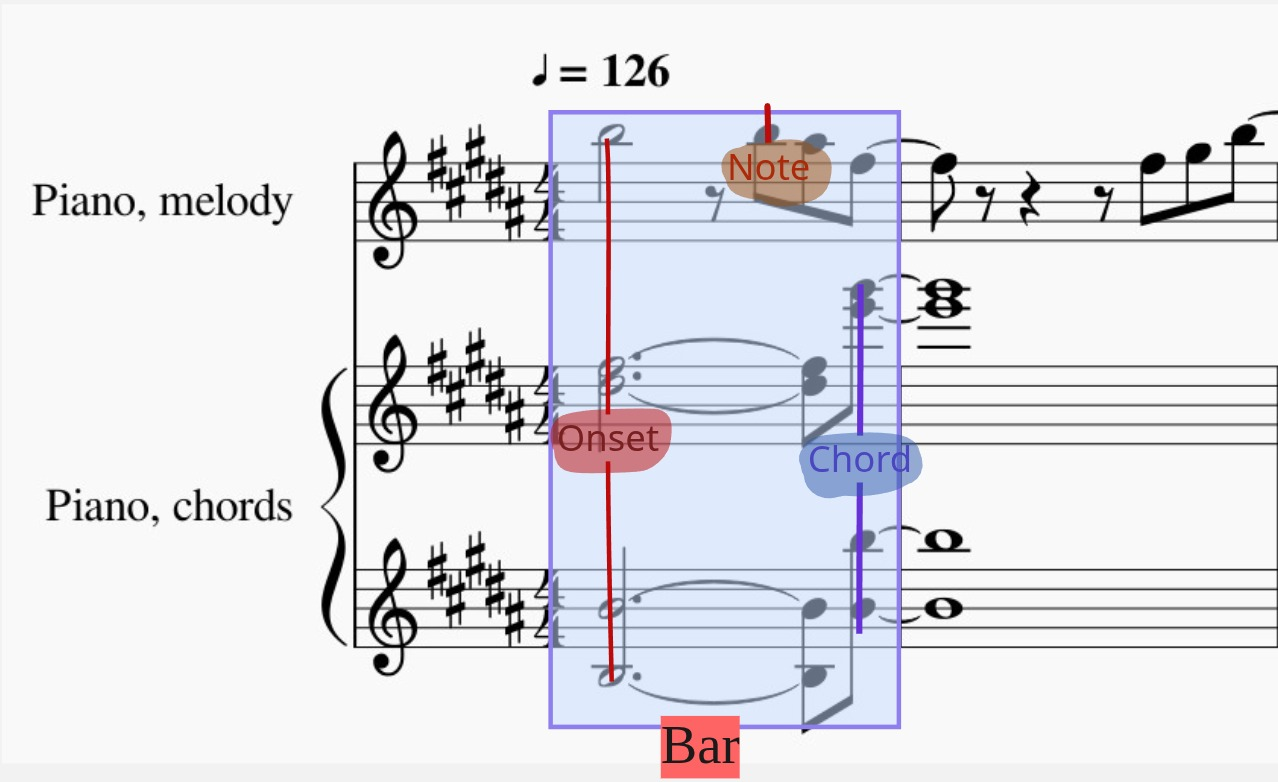
\includegraphics[width=\linewidth]{graph_hierarchy_score.jpg}
\caption{Иерархия в формате нотной записи}
\label{fig:graph-representation-score}
\end{subfigure}
\caption{Графовое представление:}
\label{fig:graph-representation}
\end{figure}

\subsection{Разведочный анализ данных}

После первичной обработки был проведён разведочный анализ корпуса. В работе используется 26175 музыкальных фрагментов, разделённых на обучающую, валидационную и тестовую подвыборки в соотношении 80\%/10\%/10\% соответственно. В общей сложности корпус содержит 449072 аккордовых события и 1338346 мелодических событий.

Основная ценность \textit{HookTheory Dataset} состоит в том, что он содержит не только нотные события, но и метаинформацию и музыкально-теоретические аннотации. К общей метаинформации относятся тональность, лад, темп и ритмическая сетка. Аккордовые события содержат ступень аккорда, тип аккорда, обращение, добавочные ступени, альтерации, задержания, признаки заимствования из другого лада, длительность и временную позицию. Мелодические события описываются ступенью лада, октавным регистром, длительностью и временной позицией.

Анализ распределений показал, что данные имеют выраженный дисбаланс по ряду признаков. В распределении тональностей заметно доминирование тональности \textit{C}, тогда как альтерированные тональности представлены существенно реже (см. \ref{fig:key-distribution}). Распределение ладов также является неравномерным: наиболее распространённые лады представлены значительно лучше, чем редкие модальные разновидности (см. \ref{fig:mode-distribution}). В рамках данной работы фрагменты в гармоническом миноре и фригийском доминантовом ладу были исключены из рассмотрения, поскольку число таких примеров недостаточно для устойчивого обучения и объективной оценки модели.

Для ритмической сетки наблюдается ожидаемое доминирование четырёхдольной пульсации. Данный дисбаланс не является критическим для поставленной задачи, поскольку основное внимание в работе уделяется не генерации ритма, а оценке мелодико-гармонической согласованности.

В аккордовых событиях заметно доминирование аккордов, построенных на первой ступени тональности (см. \ref{fig:chord-degree-distribution}). Это соответствует музыкально-теоретическим ожиданиям, поскольку тоническая функция является одной из наиболее устойчивых и частотных в тональной музыке. По типам аккордов преобладают трезвучия и септаккорды, тогда как более сложные структуры представлены значительно реже. Распределение типов аккордов представлено отдельно (см. \ref{fig:chord-type-distribution}). Среди мелодических событий также наблюдается неравномерность: диатонические ступени встречаются существенно чаще, чем альтерированные, а один из октавных регистров доминирует над остальными (см. \ref{fig:melodic-degree-distribution}).

Наличие дисбаланса является важным ограничением корпуса. Однако в данной работе он не рассматривается как ошибка данных, поскольку во многом отражает реальные статистические закономерности западной популярной музыки. Для задачи оценки музыкально-теоретической согласованности важно, чтобы модель хорошо усваивала наиболее типичные и устойчивые отношения между мелодией, аккордами и тональностью. Именно такие отношения составляют основную часть корпуса.

При этом результаты модели следует интерпретировать прежде всего в рамках наиболее представленных областей набора данных: диатонической тональности, распространённых ладов, типичных аккордовых функций, трезвучий и септаккордов. Редкие классы могут рассматриваться как направление для дальнейшего расширения корпуса и улучшения модели.

\textbf{Вывод по главе.} В данной главе был обоснован выбор \textit{HookTheory Dataset}, описан процесс его обработки и проведён разведочный анализ данных. Несмотря на наличие дисбаланса, корпус является подходящим для поставленной задачи, поскольку содержит связь между мелодией, аккордами, тональностью и метрической структурой. Это позволяет использовать его для построения графового критика, оценивающего музыкально-теоретическую согласованность \textit{MIDI}-фрагментов.

\newpage

\chapter{Постановка задачи и архитектура графового критика}

В данной главе формулируется задача построения графового критика --- модели, оценивающей музыкально-теоретическую согласованность \textit{MIDI}-фрагмента. Критик рассматривается как отдельный модуль оценки, который присваивает музыкальному фрагменту скалярную оценку. В дальнейшем такая оценка используется как награда при дообучении \textit{text2midi}-модели.

Архитектура критика строится как система из двух моделей: графового учителя и графового ученика. Учитель является более информированной моделью: на вход он получает расширенное графовое представление музыкального примера, включающее структуру музыкального фрагмента, временную сетку, ноты, аккорды и дополнительные музыкально-теоретические признаки. Ученик является более компактной моделью, предназначенной для практического применения: он работает с \textit{MIDI}-фрагментом и признаками, которые можно извлечь автоматически, после чего пытается воспроизвести оценки учителя (см. Рисункок ~\ref{fig:graph-critic-application}).

\begin{figure}[htbp]
\centering
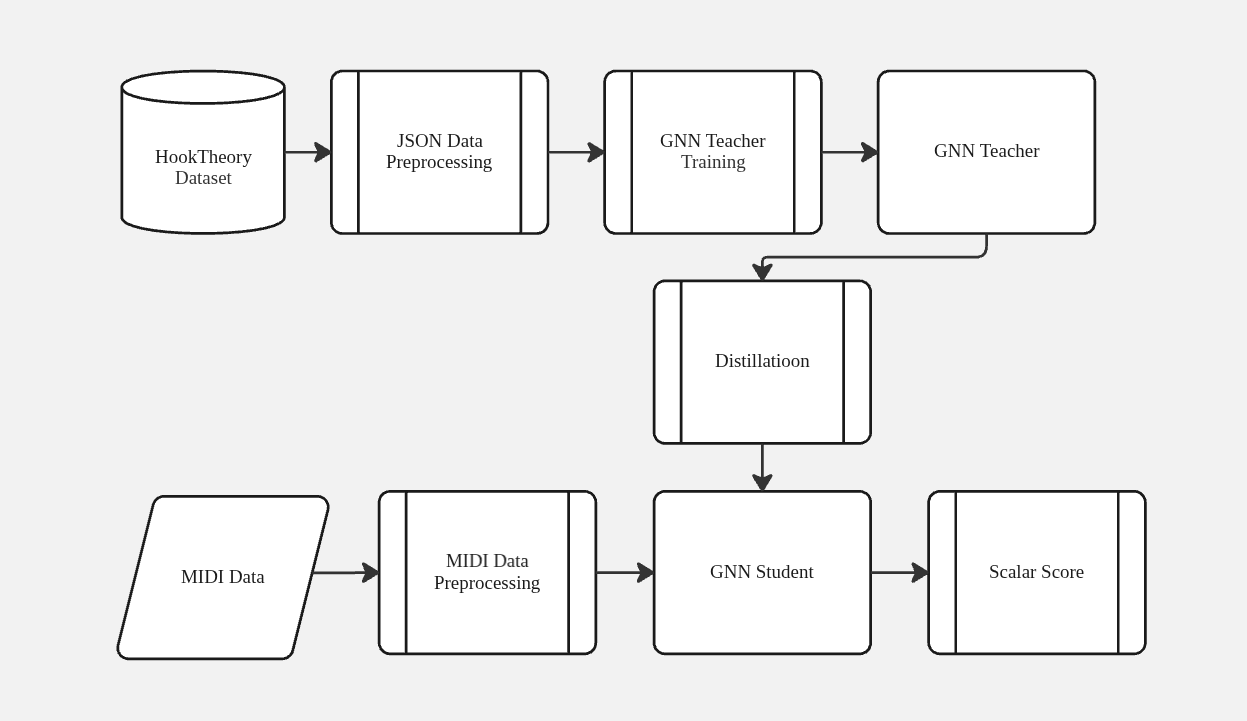
\includegraphics[width=0.94\textwidth,height=0.50\textheight,keepaspectratio]{graph_critic_application.png}
\caption{Схема применения графового критика}
\label{fig:graph-critic-application}
\end{figure}

Формально музыкальный пример представляется как гетерогенный граф:

\[
\mathcal{G}=(V,E,\tau_V,\tau_E,X),
\]

где $V$ --- множество вершин, $E$ --- множество рёбер, $\tau_V$ задаёт тип вершины, $\tau_E$ задаёт тип ребра, а $X=\{x_v\}_{v\in V}$ --- множество признаков вершин. Вершины соответствуют различным музыкальным объектам: фрагменту, тактам, временным позициям, нотам и аккордам. Рёбра описывают как иерархические связи, например принадлежность ноты временной позиции, так и последовательные связи, например переход от одной ноты или временной позиции к следующей.

Цель критика состоит в построении функции

\[
s_\theta(\mathcal{G})\in\mathbb{R},
\]

которая отображает музыкальный граф в скалярную оценку. Чем выше значение $s_\theta(\mathcal{G})$, тем более согласованным с музыкально-теоретической точки зрения считается фрагмент.

\subsection{Графовый учитель}

Графовый учитель представляет собой гетерогенную графовую нейронную сеть, обучаемую на задаче различения исходных музыкальных графов и их искусственно искажённых версий. Основная идея состоит в том, что корректный музыкальный пример должен получать более высокий \textit{score}, чем пример, в котором нарушены локальные или глобальные музыкальные связи.

Пусть для исходного графа $\mathcal{G}$ строится искажённый граф $\widetilde{\mathcal{G}}$. Тогда модель обучается выполнять условие:

\[
s_\theta(\mathcal{G}) > s_\theta(\widetilde{\mathcal{G}}).
\]

Искажения применяются к музыкальным объектам графа. Они могут включать сдвиг ноты во времени, изменение аккорда, замену локального элемента, нарушение связи между мелодией и гармонией, а также другие теоретически обоснованные искажения. Такой подход не требует внешней ручной разметки качества: пары «корректный пример --- испорченный пример» строятся автоматически, что позволяет обучать критик в \textit{self-supervised} режиме.

Поскольку вершины разных типов имеют различные признаки, сначала признаки каждой вершины проецируются в общее скрытое пространство:

\[
h_v^{(0)}=\phi_{\tau_v}(x_v),
\]

где $\phi_{\tau_v}$ --- \textit{encoder} для типа вершины $\tau_v$, реализованный как \textit{MLP}.

Далее применяется несколько слоёв гетерогенной \textit{GNN}. Для каждого типа ребра $r$ сообщения вычисляются отдельно:

\[
m_{u\to v}^{(l,r)}=W_r^{(l)}h_u^{(l)}.
\]

После этого сообщения от соседей агрегируются:

\[
m_v^{(l)}=\sum_{r\in R}\operatorname{AGG}_{u\in N_r(v)} m_{u\to v}^{(l,r)}.
\]

Состояние вершины обновляется с \textit{residual}-связью, нормализацией и нелинейностью:

\[
h_v^{(l+1)}=\operatorname{ReLU}\!\left(\operatorname{LN}\!\left(h_v^{(l)}+m_v^{(l)}\right)\right).
\]

После нескольких \textit{GNN}-слоёв модель получает контекстуализированные представления нот, аккордов, временных позиций и других узлов. Затем выполняется \textit{pooling} по типам вершин:

\[
g_t=\frac{1}{|V_t|}\sum_{v\in V_t}h_v^{(L)},
\]

где $V_t$ --- множество вершин типа $t$.

После объединения векторов разных типов получается общий \textit{embedding} графа:

\[
g=\psi\!\left(g_1\Vert g_2\Vert\ldots\Vert g_T\right),
\]

где $\Vert$ обозначает конкатенацию, а $\psi$ --- линейная проекция или \textit{MLP}. Итоговая оценка графа вычисляется \textit{scoring}-головой:

\[
s_\theta(\mathcal{G})=f_{\mathrm{score}}(g).
\]

Для обучения используется \textit{contrastive ranking loss}:

\[
\mathcal{L}_{\mathrm{rank}}=
\operatorname{softplus}\!\left(-\left(s_\theta(\mathcal{G})-s_\theta(\widetilde{\mathcal{G}})-m\right)\right),
\]

где $m$ --- \textit{margin}. Эта функция штрафует модель, если \textit{score} искажённого графа оказывается слишком близким к \textit{score} исходного графа или превосходит его.

Дополнительно может использоваться бинарная классификационная компонента:

\[
\mathcal{L}_{\mathrm{bin}}=\frac{1}{2}\left(
\operatorname{BCE}\!\left(s_\theta(\mathcal{G}),1\right)+
\operatorname{BCE}\!\left(s_\theta(\widetilde{\mathcal{G}}),0\right)
\right).
\]

Общая функция потерь учителя записывается в виде:

\[
\mathcal{L}_{\mathrm{teacher}}=
\lambda_{\mathrm{rank}}\mathcal{L}_{\mathrm{rank}}+
\lambda_{\mathrm{bin}}\mathcal{L}_{\mathrm{bin}}+
\lambda_{\mathrm{local}}\mathcal{L}_{\mathrm{local}}+
\lambda_{\mathrm{rec}}\mathcal{L}_{\mathrm{rec}}.
\]

Здесь $\mathcal{L}_{\mathrm{local}}$ отвечает за локальное обнаружение испорченных нот, аккордов или временных позиций, а $\mathcal{L}_{\mathrm{rec}}$ используется при восстановлении замаскированных музыкальных признаков. Общая схема обучения представлена ниже (см. Рисунок~\ref{fig:teacher-training-scheme}).

\begin{figure}[htbp]
\centering
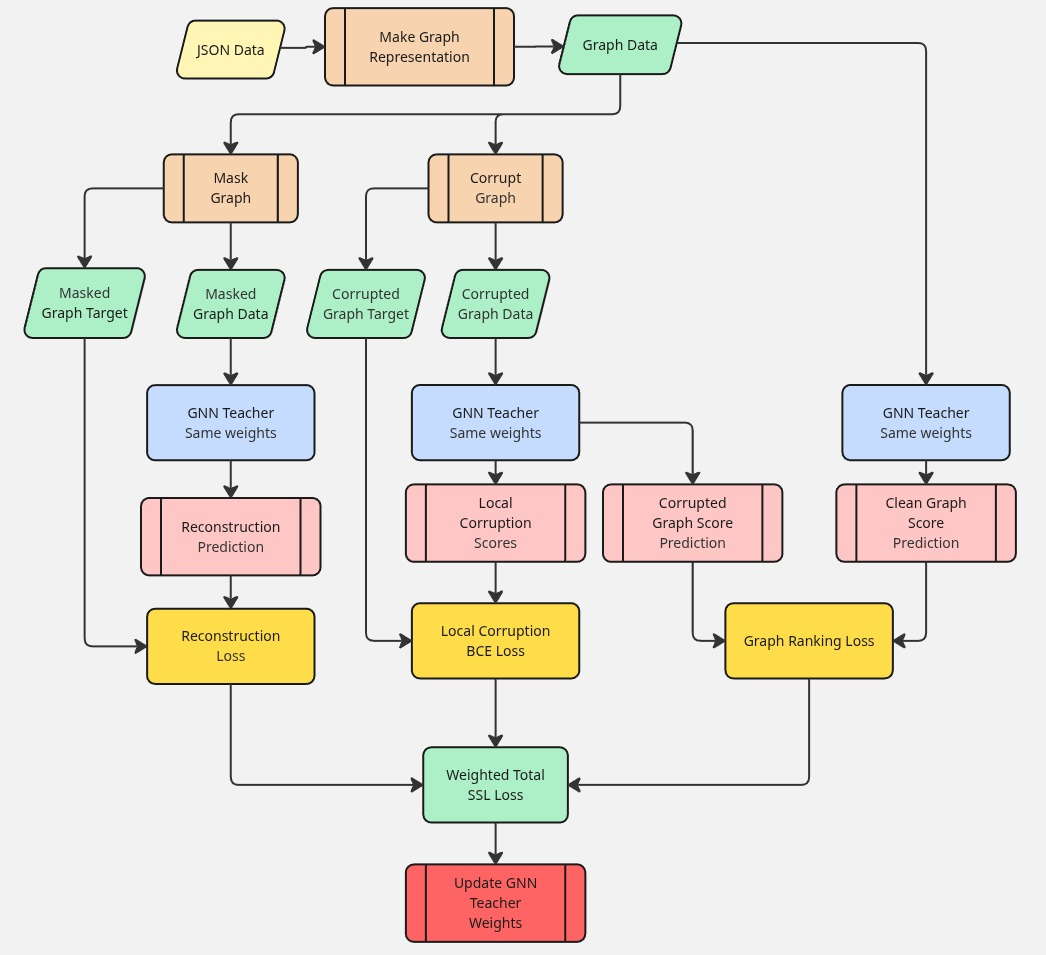
\includegraphics[width=0.8\textwidth,height=0.8\textheight,keepaspectratio]{teacher_training_scheme.jpg}
\caption{Общая схема обучения графового учителя}
\label{fig:teacher-training-scheme}
\end{figure}

\subsection{Графовый ученик}

Графовый ученик является уменьшенной и более прикладной версией графового учителя. Его основное отличие состоит в том, что он не получает расширенную информацию, доступную учителю, а работает только с \textit{MIDI}-фрагментом и автоматически извлекаемыми признаками. Это делает ученика пригодным для использования в дальнейшем цикле генерации и оценки \textit{MIDI}.

На вход ученику подаётся \textit{MIDI}-фрагмент, из которого строится граф:

\[
\mathcal{G}_M=(V_M,E_M,X_M).
\]

Вершины такого графа соответствуют базовым объектам \textit{MIDI}: фрагменту, тактам, временным позициям, нотам и предполагаемым аккордам. Рёбра задают временную и структурную организацию: такты связаны с временными позициями, временные позиции --- с нотами и аккордами, а соседние ноты и аккорды соединяются последовательными рёбрами.

Так как \textit{MIDI} не всегда содержит готовую гармоническую разметку, для ученика важен отдельный этап извлечения аккордов. Аккорд восстанавливается по набору нот, звучащих одновременно или почти одновременно в небольшом временном окне $w$. Для этого из \textit{MIDI}-событий строится множество частотных классов:

\[
P_w = \{p_i \bmod 12 \mid p_i \in w\},
\]

где $p_i$ --- \textit{MIDI высота} ноты, а операция $\bmod 12$ переводит абсолютную высоту в класс высоты. Например, ноты $C_4$, $E_4$, $G_4$, $B\flat_4$ дают множество

\[
P_w = \{C, E, G, B\flat\}.
\]

Далее перебирается множество кандидатов аккорда $c \in \mathcal{C}$. Каждый кандидат задаёт корень, тип аккорда, возможное обращение, набор основных тонов аккордового тела, а также дополнительные признаки: добавленные ступени, задержания, альтерации, пропуски и заимствованный ладовый контекст. Для кандидата строится множество частотных классов, которое он способен объяснить:

\[
B(c) = \{\text{pitch classes, входящие в тело аккорда } c\}.
\]

После этого вычисляется \textit{score} соответствия между наблюдаемыми нотами и кандидатом:

\[
q(c, P_w)
=
q_{+}(c, P_w)
-
q_{-}(c, P_w),
\]

где $q_{+}$ --- положительный вклад объяснённых признаков, а $q_{-}$ --- штрафы за несоответствия.

Положительная часть \textit{score} может быть записана как

\[
\begin{aligned}
q_{+}(c, P_w)
={}&
\lambda_1 \operatorname{mode\_match}(c)
+
\lambda_2 \operatorname{bass\_match}(c)
+
\lambda_3 |P_w \cap B(c)| \\
&+
\lambda_4 \operatorname{explained\_extras}(c, P_w).
\end{aligned}
\]
\newpage
Интерпретация компонент положительной части \textit{score} приведена в Таблице~\ref{tab:positive-score-components}.

\begin{table}[htbp]
\caption{Компоненты положительной части аккордового \textit{score}}
\label{tab:positive-score-components}
\centering
\footnotesize
\begin{tabular}{@{}p{0.34\textwidth}p{0.58\textwidth}@{}}
\toprule
\textit{Компонента} & \textit{Интерпретация} \\
\midrule
$\operatorname{mode\_match}(c)$ & Поощряет кандидата, если его ладовый контекст совпадает с основным контекстом фрагмента. \\
$\operatorname{bass\_match}(c)$ & Поощряет совпадение басовой ноты с ожидаемым басом аккорда или его обращением. \\
$|P_w \cap B(c)|$ & Показывает, сколько наблюдаемых \textit{pitch classes} объясняется телом аккорда. \\
$\operatorname{explained\_extras}(c, P_w)$ & Учитывает дополнительные ноты, которые не входят в простое трезвучие, но могут быть объяснены как септима, нона, задержание или альтерация. \\
\bottomrule
\end{tabular}
\end{table}

Штрафная часть имеет вид

\[
\begin{aligned}
q_{-}(c, P_w)
={}&
\mu_1 |\operatorname{Unexplained}(c, P_w)|
+
\mu_2 |\operatorname{MissingCore}(c, P_w)| \\
&+
\mu_3 \operatorname{borrowed\_mode\_penalty}(c)
+
\mu_4 \operatorname{mode\_distance}(c) \\
&+
\mu_5 \operatorname{body\_size\_penalty}(c)
+
\mu_6 \operatorname{complexity\_penalty}(c).
\end{aligned}
\]

Интерпретация компонент штрафной части \textit{score} приведена в Таблице~\ref{tab:negative-score-components}.

\begin{table}[htbp]
\caption{Компоненты штрафной части аккордового \textit{score}}
\label{tab:negative-score-components}
\centering
\footnotesize
\resizebox{\textwidth}{!}{%
\begin{tabular}{@{}p{0.38\textwidth}p{0.56\textwidth}@{}}
\toprule
\textit{Компонента} & \textit{Интерпретация} \\
\midrule
$\operatorname{Unexplained}(c, P_w)$ & Наблюдаемые \textit{pitch classes}, которые кандидат не может объяснить. \\
$\operatorname{MissingCore}(c, P_w)$ & Обязательные тона аккорда, отсутствующие в \textit{MIDI}-окне. \\
$\operatorname{borrowed\_mode\_penalty}(c)$ & Штрафует за использование заимствованного лада без достаточных оснований. \\
$\operatorname{mode\_distance}(c)$ & Учитывает удалённость кандидата от текущего ладового контекста. \\
$\operatorname{body\_size\_penalty}(c)$ & Не даёт модели выбирать чрезмерно сложные аккорды без необходимости. \\
$\operatorname{complexity\_penalty}(c)$ & Объединяет штрафы за добавленные ступени, задержания, альтерации и пропущенные обязательные тона. \\
\bottomrule
\end{tabular}%
}
\end{table}

Итоговый кандидат выбирается по максимуму:

\[
\hat{c}
=
\arg\max_{c \in \mathcal{C}}
q(c, P_w).
\]
\newpage
Например, пусть в момент времени $t$ наблюдаются \textit{MIDI}-ноты:

\[
C - E - G - B\flat.
\]

Тогда

\[
P_t = \{C, E, G, B\flat\}.
\]

Рассмотрим несколько кандидатов.

\textbf{Кандидат 1: $C7$.}

\[
B(C7)=\{C,E,G,B\flat\}.
\]

Этот кандидат объясняет все наблюдаемые \textit{pitch classes}:

\[
P_t \cap B(C7)=\{C,E,G,B\flat\}.
\]

У него нет отсутствующих основных тонов и нет необъяснённых нот:

\[
\operatorname{MissingCore}(C7, P_t)=\varnothing,
\quad
\operatorname{Unexplained}(C7, P_t)=\varnothing.
\]

Поэтому \textit{score} будет высоким: модель видит полный доминантсептаккорд без лишних нот.

\textbf{Кандидат 2: $C$ major.}

\[
B(C)=\{C,E,G\}.
\]

Этот кандидат хорошо объясняет трезвучие $C,E,G$, но не объясняет $B\flat$:

\[
\operatorname{Unexplained}(C, P_t)=\{B\flat\}.
\]

Если $B\flat$ не интерпретируется как допустимая добавленная или альтерированная ступень, кандидат получает штраф за лишнюю необъяснённую ноту. Поэтому его \textit{score} ниже, чем у $C7$.

\textbf{Кандидат 3: $Am7\flat5/C$.}

Такой кандидат может иметь тело

\[
B(Am7\flat5)=\{A,C,E\flat,G\}.
\]

В наблюдаемых нотах есть $C$ и $G$, но отсутствуют важные для этого кандидата $A$ и $E\flat$, а вместо $E\flat$ наблюдается $E$. Тогда возникают одновременно пропущенные основные тона и несовпадающие высотные классы:

\[
\operatorname{MissingCore}(Am7\flat5/C, P_t)=\{A,E\flat\},
\]

а часть наблюдаемых нот плохо согласуется с телом кандидата. Несмотря на возможное совпадение баса $C$, общий \textit{score} оказывается ниже, чем у $C7$.

Таким образом, алгоритм выбирает не просто самый большой аккорд и не просто ближайшее трезвучие, а кандидата, который лучше всего объясняет наблюдаемые \textit{MIDI}-ноты при минимальном числе лишних допущений. В приведённом примере итоговое предсказание будет

\[
\hat{c}=C7.
\]

Такая оценка важна для графового ученика, потому что предсказанный аккорд затем превращается в вершину графа и влияет на признаки гармонического контекста, связи между нотами и аккордами, а также на итоговую оценку \textit{MIDI}-фрагмента.

После построения \textit{MIDI}-графа ученик использует компактную гетерогенную \textit{GNN}. Для каждой вершины строится начальное представление:

\[
z_v^{(0)}=\phi_{\tau_v}(x_v),
\]

после чего несколько графовых слоёв обновляют его через сообщения от соседей:

\[
z_v^{(l+1)}=\sigma\!\left(\operatorname{LN}\!\left(
z_v^{(l)}+\sum_r\operatorname{AGG}_{u\in N_r(v)}W_r^{(l)}z_u^{(l)}
\right)\right).
\]

Далее применяется \textit{pooling} по вершинам и строится \textit{embedding} \textit{MIDI}-графа:

\[
z_G=\operatorname{Pool}\!\left(\{z_v^{(L)}\}_{v\in V_M}\right).
\]

Итоговая оценка ученика равна:

\[
s_\varphi(\mathcal{G}_M)=f_{\mathrm{student}}(z_G).
\]

Ученик обучается не на ручных метках, а на оценках учителя. Если учитель присваивает музыкальному фрагменту \textit{score} $s_\theta(\mathcal{G})$, то ученик минимизирует ошибку дистилляции:

\[
\mathcal{L}_{\mathrm{distill}}=
\left|s_\varphi(\mathcal{G}_M)-s_\theta(\mathcal{G})\right|,
\]

или её сглаженный вариант:

\[
\mathcal{L}_{\mathrm{distill}}=
\operatorname{SmoothL1}\!\left(s_\varphi(\mathcal{G}_M),s_\theta(\mathcal{G})\right).
\]

Для пар \textit{clean/corrupted} дополнительно используется \textit{ranking loss}:

\[
\mathcal{L}_{\mathrm{student\text{-}rank}}=
\operatorname{softplus}\!\left(-\left(s_\varphi(\mathcal{G}_M)-s_\varphi(\widetilde{\mathcal{G}}_M)\right)\right).
\]

Эта компонента нужна для того, чтобы ученик не только приближал абсолютные оценки учителя, но и сохранял порядок предпочтений между корректными и искажёнными музыкальными примерами. Ниже представлена общая схема обучения графового ученика (см. Рисунок~\ref{fig:student-training-scheme}).

\begin{figure}[htbp]
\centering
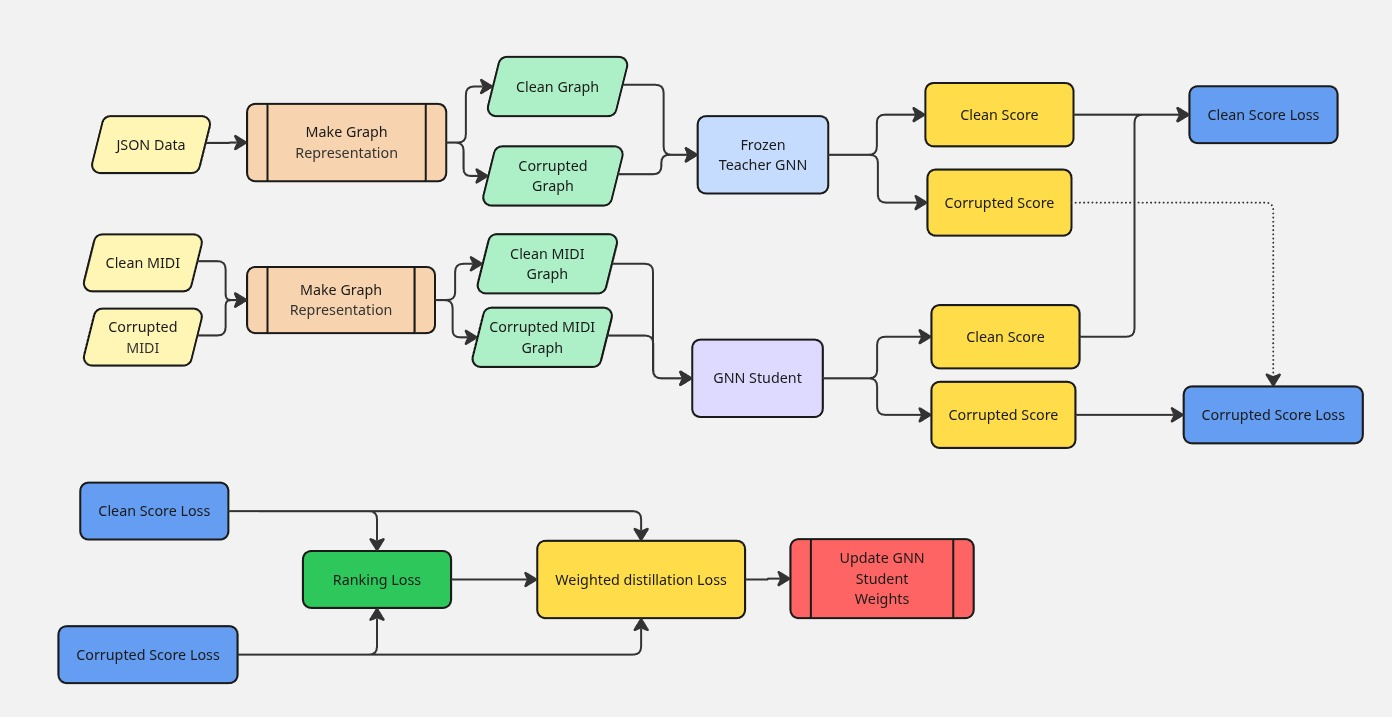
\includegraphics[width=0.94\textwidth,height=0.42\textheight,keepaspectratio]{student_training_scheme.jpg}
\caption{Общая схема обучения графового ученика}
\label{fig:student-training-scheme}
\end{figure}

\subsection{Эксперименты графового учителя}

Перед описанием отдельных экспериментов зафиксируем общую схему оценки. Экспериментальная часть состоит из двух блоков: сначала проверяется графовый учитель, который получает расширенный музыкально-теоретический граф, затем оценивается графовый ученик, работающий только с \textit{MIDI}-представлением. В таблицах используются метрики качества ранжирования, восстановления аккордов и дистилляции \textit{score}-функции.

Для оценки учительской-модели использовались следующие базовые \textit{ranking}-метрики:

\[
\operatorname{IntraAcc}=\frac{1}{N}\sum_{i=1}^{N}
\mathbf{1}\!\left[s(\mathcal{G}_i)>s(\widetilde{\mathcal{G}}_i)\right],
\]

\[
\operatorname{InterAcc}=\frac{1}{N(N-1)}\sum_{i\ne j}
\mathbf{1}\!\left[s(\mathcal{G}_i)>s(\widetilde{\mathcal{G}}_j)\right],
\]

\[
\operatorname{RankAcc}=\frac{1}{N^2}\sum_{i,j}
\mathbf{1}\!\left[s(\mathcal{G}_i)>s(\widetilde{\mathcal{G}}_j)\right].
\]

Здесь $\mathcal{G}_i$ --- исходный граф, $\widetilde{\mathcal{G}}_i$ --- его искажённая версия, а $s(\cdot)$ --- \textit{score} графового критика. Метрика \textit{IntraAcc} показывает долю правильно упорядоченных пар \textit{clean/corrupted} внутри одного примера, \textit{InterAcc} сравнивает исходные графы с искажениями других примеров, а \textit{RankAcc} объединяет все такие сравнения внутри оцениваемого набора. Префикс \textit{Best} означает лучшее значение за время обучения.

Остальные метрики и служебные показатели, используемые в таблицах экспериментов, имеют следующую интерпретацию:

\begin{itemize}
\item \textit{BinaryAcc} --- точность бинарного различения исходных и искажённых графов после порогового решения по \textit{score} или логиту модели.
\item \textit{SuccessRate} --- доля случаев, где исходный граф получает более высокий \textit{score}, чем его \textit{OOD}-преобразование; \textit{Mean gap} --- средняя разность $s(\mathcal{G})-s(\mathcal{G}')$; \textit{Global RankAcc} --- ранжировочная точность на всём наборе \textit{OOD}-пар.
\item \textit{Applied samples} --- число примеров, к которым удалось применить искажение или преобразование; \textit{Applied rate} --- соответствующая доля от проверяемого набора.
\item \textit{Top-1 exact} --- доля случаев полного совпадения предсказанного аккорда с разметкой; \textit{Top-5 contains GT} --- доля случаев, где правильный аккорд входит в пять лучших кандидатов.
\item \textit{Root acc}, \textit{Type acc}, \textit{Root+Type acc}, \textit{Mode acc} и \textit{Inversion acc} оценивают соответственно правильность корня аккорда, типа аккорда, их совместного совпадения, ладового контекста и обращения.
\item \textit{Manual weights} и \textit{Learned weights} в таблице по типам аккордов показывают точность восстановления внутри конкретного класса аккордов при ручных и обучаемых весах \textit{scoring}-функции.
\item \textit{Pair rank acc} --- доля корректно упорядоченных пар \textit{clean/corrupted} для \textit{student}/\textit{observer}; \textit{Batch rank acc} --- доля корректных сравнений между всеми положительными и отрицательными примерами внутри батча.
\item \textit{Spearman} --- ранговая корреляция между оценками \textit{student} и \textit{teacher}; \textit{Pearson} --- линейная корреляция между этими оценками.
\item \textit{MAE} --- средняя абсолютная ошибка между \textit{score} ученика и учителя; \textit{Score distill loss} --- значение функции потерь дистилляции для скалярного \textit{score}. Для метрик со стрелкой $\uparrow$ лучше большее значение, а для метрик со стрелкой $\downarrow$ --- меньшее.
\end{itemize}

Эксперименты графового учителя направлены на проверку того, способен ли \textit{teacher} различать исходные и искажённые музыкальные графы, а также какие архитектурные и обучающие модификации повышают качество ранжирования.

\subsubsection{\textit{Smoke}-тесты и ранние \textit{one-batch ablation}}

Первый этап экспериментов представлял собой \textit{smoke}-тесты и ранние \textit{one-batch ablation}. Его цель состояла не в финальной оценке качества, а в проверке работоспособности \textit{contrastive}-пайплайна. Для каждого исходного графа строилась искажённая версия, после чего модель обучалась выполнять условие $s_\theta(\mathcal{G})>s_\theta(\widetilde{\mathcal{G}})$. На этом этапе сравнивались простые \textit{graph corruptions} и более содержательные \textit{theory-aware corruptions}. Результаты приведены в Таблице~\ref{tab:1}.

\begin{table}[htbp]
\caption{\textit{Smoke}-тесты и ранние \textit{one-batch ablation}}
\label{tab:1}
\centering
\footnotesize
\resizebox{\textwidth}{!}{%
\begin{tabular}{@{}lllll@{}}
\toprule
\textit{Corruption family} & \textit{Pooling} & \textit{Hybrid scorer} & \textit{Epochs} & \textit{Best rank acc} $\uparrow$ \\
\midrule
\textit{Theory-aware ablation} & \textit{mean\_max} & \textit{true} & 500 & \textbf{1.0000} \\
\textit{Theory-aware ablation} & \textit{mean\_max} & \textit{false} & 500 & \textbf{1.0000} \\
\textit{Theory-aware ablation} & \textit{mean} & \textit{true} & 500 & \textbf{1.0000} \\
\textit{Theory-aware ablation} & \textit{mean} & \textit{false} & 500 & \textbf{1.0000} \\
\textit{Graph ablation} & \textit{mean\_max} & \textit{true} & 500 & 0.8750 \\
\textit{Graph ablation} & \textit{mean} & \textit{true} & 500 & 0.8750 \\
\textit{Graph ablation} & \textit{mean} & \textit{false} & 500 & 0.8750 \\
\textit{Graph ablation} & \textit{mean\_max} & \textit{false} & 500 & 0.6875 \\
\bottomrule
\end{tabular}%
}
\end{table}

Результаты показали, что на раннем \textit{sanity-check} уровне \textit{theory-aware corruptions} дают более устойчивое поведение: лучшая метрика \textit{rank acc} достигала 1.0000 во всех конфигурациях, тогда как простые \textit{graph corruptions} давали менее стабильный результат. Это стало основанием использовать музыкально осмысленные искажения в дальнейших экспериментах.

\subsubsection{Обобщение на \textit{OOD-corruptions}}

Дополнительно была проверена обобщающая способность графового критика на искажениях, которые не совпадают напрямую с основным набором обучающих искажений. Цель эксперимента состояла в проверке двух гипотез. Во-первых, если новое искажение действительно ухудшает музыкальный фрагмент, то учительская-модель должна понижать его \textit{score} даже без прямого обучения на таком типе ошибки. Во-вторых, если преобразование является условно безвредным, то оно не должно превращаться для модели в ложный отрицательный сигнал.

Для исходного графа $\mathcal{G}_i$ и его преобразованной версии $\mathcal{G}'_i$ рассматривалась разность \textit{score}:

\[
\Delta_i=s(\mathcal{G}_i)-s(\mathcal{G}'_i).
\]

Если $\Delta_i>0$, то модель оценивает исходный граф выше преобразованного. Для вредных \textit{OOD-corruptions} это считается правильной реакцией, а для безвредных преобразований систематически положительный \textit{gap}, наоборот, был бы признаком лишнего шума. Основная метрика записывается как

\[
\operatorname{SuccessRate}=
\frac{1}{N}
\sum_{i=1}^{N}
\mathbf{1}\!\left[s(\mathcal{G}_i)>s(\mathcal{G}'_i)\right].
\]

Также оценивался средний \textit{gap}:

\[
\overline{\Delta}=
\frac{1}{N}
\sum_{i=1}^{N}
\left(s(\mathcal{G}_i)-s(\mathcal{G}'_i)\right).
\]

Результаты приведены в Таблице~\ref{tab:ood-corruption-groups}.

\begin{table}[htbp]
\caption{Проверка обобщения \textit{teacher}-модели на \textit{OOD-corruptions}}
\label{tab:ood-corruption-groups}
\centering
\footnotesize
\resizebox{\textwidth}{!}{%
\begin{tabular}{@{}p{3.6cm}rrrrp{5.1cm}@{}}
\toprule
\textit{Group} & \textit{Applied samples} & \textit{SuccessRate} & \textit{Mean gap} & \textit{Global RankAcc} & \textit{Interpretation} \\
\midrule
\textit{Harmful OOD corruptions} & 4265 & 0.6080 & 0.6649 & 0.5504 & Новые вредные искажения в среднем понижают \textit{score} \\
\textit{Benign transformations} & 1763 & 0.5230 & 0.0110 & 0.5012 & Безвредные преобразования почти не создают систематический штраф \\
\bottomrule
\end{tabular}
}
\end{table}

Отдельные типы вредных \textit{OOD}-искажений давали особенно выраженный сигнал. Например, \texttt{strong\_weak\_beat\_flip} достиг \textit{SuccessRate} $=0.7859$ и среднего \textit{gap} $=4.9666$, то есть модель хорошо распознаёт нарушение метрически сильных и слабых долей. Удаление ноты из \textit{onset} также давало устойчивый эффект: \textit{SuccessRate} $=0.7594$. Удаление аккорда из \textit{onset} имело \textit{SuccessRate} $=0.7282$ и средний \textit{gap} $=0.4860$.

При этом более тонкие искажения, например локальный сдвиг фрагмента на полутон, нарушение октавного скачка или изменение длительности ноты, давали более слабый сигнал: их \textit{SuccessRate} находился ближе к 0.5. Это показывает, что критик лучше обобщает на структурно и гармонически выраженные ошибки, чем на очень локальные или неоднозначные изменения.

\begin{table}[htbp]
\caption{Примеры вредных \textit{OOD-corruptions}}
\label{tab:ood-harmful-examples}
\centering
\footnotesize
\begin{tabular}{@{}p{7.0cm}rrr@{}}
\toprule
\textit{OOD corruption} & \textit{Applied rate} & \textit{SuccessRate} $\uparrow$ & \textit{Mean gap} $\uparrow$ \\
\midrule
\texttt{strong\_weak\_beat\_flip} & 0.906 & \textbf{0.7859} & \textbf{4.9666} \\
\texttt{drop\_note\_from\_onset} & 0.906 & 0.7594 & 0.0096 \\
\texttt{drop\_chord\_from\_onset} & 0.986 & 0.7282 & 0.4860 \\
\texttt{out\_of\_key\_note} & 0.906 & 0.5850 & 0.0507 \\
\texttt{semitone\_from\_bass\_or\_chord\_tone} & 0.902 & 0.5676 & 0.0610 \\
\bottomrule
\end{tabular}
\end{table}

Отдельно важен результат на безвредных преобразованиях. Для группы \textit{benign transformations} средний \textit{gap} оказался практически нулевым: 0.0110, а \textit{Global RankAcc} $=0.5012$, то есть почти совпал со случайным уровнем. Это означает, что \textit{teacher}-модель не начинает автоматически штрафовать любое изменение \textit{MIDI}-графа. Например, транспозиция с соответствующим изменением тоники дала \textit{SuccessRate} $=0.4580$ и средний \textit{gap}, близкий к 0.0000, что соответствует ожидаемому поведению: музыкально эквивалентное преобразование не должно восприниматься как ошибка.

Таким образом, эксперимент показывает, что механизм искажающего-обучения не сводится к запоминанию конкретных типов обучающих искажений. Финальный учитель частично обобщает \textit{learned scoring} на новые вредные нарушения, но при этом не превращает нейтральные музыкальные преобразования в дополнительный шумный отрицательный сигнал.

\subsubsection{Влияние локального \textit{attention}-контекста}

Следующий этап был направлен на проверку влияния локального \textit{attention}-контекста. Для локального контекста сравнивались \textit{mean}-агрегация и \textit{attention}-механизм. Результаты приведены в Таблице~\ref{tab:2}.

\begin{table}[htbp]
\caption{\textit{Attention/local context ablation}}
\label{tab:2}
\centering
\footnotesize
\resizebox{\textwidth}{!}{%
\begin{tabular}{@{}llllllll@{}}
\toprule
\textit{Pooling} & \textit{Local context} & \textit{Hidden / layers} & \textit{MLM / corr epochs} & \textit{RankAcc} $\uparrow$ & \textit{IntraAcc} $\uparrow$ & \textit{InterAcc} $\uparrow$ & \textit{BinaryAcc} $\uparrow$ \\
\midrule
\textit{mean\_max} & \textit{mean} & 128 / 3 & 3 / 7 & 0.8081 & 0.8134 & 0.8078 & 0.7400 \\
\textit{mean\_max} & \textit{attention} & 128 / 3 & 3 / 7 & \textbf{0.8133} & \textbf{0.8293} & \textbf{0.8125} & 0.7407 \\
\textit{attention} & \textit{mean} & 128 / 3 & 3 / 7 & 0.8047 & 0.7704 & 0.8058 & 0.7301 \\
\textit{attention} & \textit{attention} & 128 / 3 & 3 / 7 & 0.8076 & 0.7763 & 0.8087 & \textbf{0.7425} \\
\bottomrule
\end{tabular}%
}
\end{table}

Лучшей конфигурацией по основным \textit{ranking}-метрикам стала комбинация \textit{mean\_max pooling} и \textit{attention local context}. Это показывает, что \textit{attention} оказывается полезен именно в локальном контексте, где модель должна определить, какие соседние ноты, аккорды и \textit{onset}-узлы важны для обнаружения музыкального нарушения.

\subsubsection{Поэтапное обучение}

Для более честного сравнения в последующих экспериментах был использован фиксированный набор \textit{corruption}-пар:

\[
D_{\mathrm{pairs}}=\{(\mathcal{G}_i,\widetilde{\mathcal{G}}_i)\}_{i=1}^{N}.
\]

Это позволило сравнивать разные режимы обучения на одном и том же наборе отрицательных примеров. 

Далее проверялось влияние поэтапного обучения. Обучение делилось на две стадии. На первой стадии модель восстанавливала замаскированные признаки нот и аккордов, а на второй стадии включалось \textit{contrastive}-обучение на \textit{corruption}-парах. Сравнивались обучение \textit{corruption-stage} с нуля и \textit{staged}-вариант, в котором модель сначала проходила \textit{MLM}-предобучение, а затем дообучалась на \textit{corruption}-парах. Результаты представлены в Таблице~\ref{tab:3}.

\begin{table}[htbp]
\caption{\textit{Staged training}}
\label{tab:3}
\centering
\scriptsize
\resizebox{\textwidth}{!}{%
\begin{tabular}{@{}llllllllll@{}}
\toprule
\textit{Training mode} & \textit{Init} & \textit{Hidden / layers} & \textit{Pooling} & \textit{Local context} & \textit{Corr epochs} & \textit{Best RankAcc} $\uparrow$ & \textit{Best IntraAcc} $\uparrow$ & \textit{Best InterAcc} $\uparrow$ & \textit{BinaryAcc} $\uparrow$ \\
\midrule
\textit{MLM} $\to$ \textit{corruption} & \textit{MLM checkpoint} & 128 / 3 & \textit{mean\_max} & \textit{attention} & 84 & \textbf{0.8998} & \textbf{0.9118} & \textbf{0.8994} & 0.7486 \\
\textit{Corruption from scratch} & \textit{random} & 128 / 3 & \textit{mean\_max} & \textit{attention} & 84 & 0.8963 & 0.9007 & 0.8962 & \textbf{0.7489} \\
\bottomrule
\end{tabular}%
}
\end{table}

\textit{MLM}-предобучение дало небольшой выигрыш по лучшим \textit{ranking}-метрикам: \textit{Best RankAcc} вырос с 0.8963 до 0.8998, \textit{Best IntraAcc} --- с 0.9007 до 0.9118, а \textit{Best InterAcc} --- с 0.8962 до 0.8994. При этом обучение с нуля оказалось сопоставимым и немного лучше по \textit{BinaryAcc}. Поэтому преимущество \textit{MLM}-предобучения следует интерпретировать осторожно: оно полезно как способ стабилизации обучения, но не является универсально лучшим по всем метрикам.

\subsubsection{Архитектурные модификации}

Далее были проверены архитектурные модификации: \textit{HGT-backbone}, динамическое взвешивание \textit{loss}-компонент и \textit{learned logit fusion}. Динамическое взвешивание задавалось через обучаемые параметры неопределённости:

\[
\mathcal{L}_{\mathrm{dyn}}=\sum_i\left(e^{-s_i}\mathcal{L}_i+s_i\right),
\]

где $s_i$ --- обучаемый параметр для $i$-й компоненты функции потерь. \textit{Learned logit fusion} объединял глобальный \textit{score} графа и локальные \textit{summary}-признаки:

\[
s_{\mathrm{final}}=f_{\mathrm{fusion}}\!\left(s_{\mathrm{global}}\Vert r_{\mathrm{local}}\right).
\]

Результаты \textit{ablation} приведены в Таблице~\ref{tab:4}.

\begin{table}[htbp]
\caption{\textit{Feature ablation}: \textit{dynamic weighting}, \textit{HGT} и \textit{learned logit fusion}}
\label{tab:4}
\centering
\scriptsize
\resizebox{\textwidth}{!}{%
\begin{tabular}{@{}llllllllll@{}}
\toprule
\textit{Variant} & \textit{Backbone} & \textit{Dynamic weights} & \textit{Logit fusion} & \textit{Hidden / layers} & \textit{MLM / corr epochs} & \textit{Best RankAcc} $\uparrow$ & \textit{Best IntraAcc} $\uparrow$ & \textit{Best InterAcc} $\uparrow$ & \textit{BinaryAcc} $\uparrow$ \\
\midrule
\textit{Baseline} & \textit{SAGE} & \textit{no} & \textit{no} & 128 / 3 & 20 / 40 & 0.8476 & \textbf{0.8547} & 0.8472 & 0.7668 \\
\textit{HGT} & \textit{HGT} & \textit{no} & \textit{no} & 128 / 3 & 20 / 40 & 0.8409 & 0.8410 & 0.8409 & 0.7537 \\
\textit{Dynamic weights} & \textit{SAGE} & \textit{yes} & \textit{no} & 128 / 3 & 20 / 40 & 0.8495 & 0.8530 & 0.8494 & 0.7731 \\
\textit{Learned logit fusion} & \textit{SAGE} & \textit{no} & \textit{yes} & 128 / 3 & 20 / 40 & \textbf{0.8519} & 0.8408 & \textbf{0.8523} & \textbf{0.7761} \\
\bottomrule
\end{tabular}%
}
\end{table}

Эксперименты показали, что \textit{HGT-backbone} не улучшил качество относительно \textit{SAGE-backbone}. Наиболее полезными оказались \textit{dynamic weighting} и \textit{learned logit fusion}. \textit{Dynamic weighting} улучшил баланс между компонентами функции потерь, а \textit{learned logit fusion} дал более устойчивое качество по \textit{ranking}- и \textit{binary}-метрикам.

\subsubsection{Финальная \textit{teacher}-конфигурация}

Финальная \textit{teacher}-конфигурация объединяла наиболее удачные решения: \textit{SAGE-backbone}, увеличенную скрытую размерность, четыре \textit{GNN}-слоя, \textit{local attention context}, \textit{dynamic loss weighting} и \textit{learned fusion}.

\begin{table}[htbp]
\caption{Финальная \textit{teacher}-конфигурация}
\label{tab:5}
\centering
\scriptsize
\resizebox{\textwidth}{!}{%
\begin{tabular}{@{}llllllllllll@{}}
\toprule
\textit{Teacher variant} & \textit{Backbone} & \textit{Dynamic weights} & \textit{Logit fusion} & \textit{Hidden / layers} & \textit{Pooling} & \textit{Local context} & \textit{MLM / corr epochs} & \textit{Best RankAcc} $\uparrow$ & \textit{Best IntraAcc} $\uparrow$ & \textit{Best InterAcc} $\uparrow$ & \textit{BinaryAcc} $\uparrow$ \\
\midrule
\textit{Final local-theory dynfusion} & \textit{SAGE} & \textit{yes} & \textit{yes} & 256 / 4 & \textit{mean\_max} & \textit{attention} & 30 / 39 & \textbf{0.9249} & \textbf{0.9275} & \textbf{0.9250} & \textbf{0.8456} \\
\bottomrule
\end{tabular}%
}
\end{table}

Финальный \textit{local-theory dynfusion teacher} показал наиболее сильные результаты по всем основным \textit{ranking}-метрикам. Модель достигла \textit{Best RankAcc} $=0.9249$, \textit{Best IntraAcc} $=0.9275$ и \textit{Best InterAcc} $=0.9250$. Это означает, что \textit{teacher} корректно ранжирует не только \textit{clean/corrupted}-пары одного примера, но и сохраняет преимущество \textit{clean}-графов при сравнении с \textit{corrupted}-графами других примеров внутри \textit{batch}. Дополнительно \textit{BinaryAcc} $=0.8456$ показывает, что модель научилась отделять \textit{clean} и \textit{corrupted} графы не только относительно, но и в абсолютной шкале \textit{score}.

\subsection{Эксперименты графового ученика}

Эксперименты графового ученика проверяют, насколько эффективно \textit{observer}/\textit{student}-модель восстанавливает признаки из \textit{MIDI} и воспроизводит оценки финального \textit{teacher}. В отличие от учителя, ученик не получает готовый расширенный граф, поэтому качество автоматического извлечения аккордов и дистилляции напрямую влияет на итоговую пригодность модели как \textit{reward}-критика для \textit{MIDI}-фрагментов.

\subsubsection{Качество предсказания аккордов из \textit{MIDI}}

Так как \textit{observer}-модель получает на вход только \textit{MIDI}, важным этапом является восстановление аккордовых признаков. Для каждого \textit{harmonic onset} строится множество звучащих \textit{pitch classes}:

\[
P_t
=
\{p_i \bmod 12 \mid \mathrm{note}_i \text{ звучит в момент } t\}.
\]

Для каждого кандидата аккорда $c$ вычисляется \textit{score}:

\[
\begin{aligned}
q(c, P_t)
={}&
w_{match}\operatorname{match}(c, P_t)
-
w_{miss}\operatorname{missing}(c, P_t) \\
&-
w_{extra}\operatorname{extra}(c, P_t)
-
w_{complex}\operatorname{complexity}(c).
\end{aligned}
\]

В ручном варианте веса задавались эвристически. В \textit{learned}-варианте веса подбирались по данным, после чего кандидат выбирался как

\[
\hat{c}_t
=
\arg\max_c q(c, P_t).
\]

Эксперимент \texttt{manual\_vs\_learned\_fast\_probe} сравнивал ручной \textit{scoring} и \textit{learned scoring} на задаче восстановления аккордов. Результаты приведены в Таблице~\ref{tab:chord-prediction-scoring}.

\begin{table}[htbp]
\caption{Сравнение ручного и обучаемого \textit{scoring} для восстановления аккордов из \textit{MIDI}}
\label{tab:chord-prediction-scoring}
\centering
\scriptsize
\resizebox{\textwidth}{!}{%
\begin{tabular}{@{}lrrrrrrr@{}}
\toprule
\textit{Scoring} & \textit{Top-1 exact} $\uparrow$ & \textit{Top-5 contains GT} $\uparrow$ & \textit{Root acc} $\uparrow$ & \textit{Type acc} $\uparrow$ & \textit{Root+Type acc} $\uparrow$ & \textit{Mode acc} $\uparrow$ & \textit{Inversion acc} $\uparrow$ \\
\midrule
\textit{Learned weights} & \textbf{0.9216} & \textbf{0.9907} & \textbf{0.9753} & \textbf{0.9864} & \textbf{0.9690} & \textbf{0.9324} & \textbf{0.9811} \\
\textit{Manual} & 0.7641 & 0.9184 & 0.9249 & 0.8368 & 0.8147 & 0.9061 & 0.9213 \\
\bottomrule
\end{tabular}%
}
\end{table}

Обученные веса существенно улучшили восстановление аккордов. Наиболее заметный прирост наблюдается для типа аккорда: \textit{Type acc} вырос с 0.8368 до 0.9864. Также сильно выросла точность полного совпадения: \textit{Top-1 exact} увеличился с 0.7641 до 0.9216.

Дополнительно был проведён анализ качества предсказания в зависимости от типа аккорда. Результаты представлены в Таблице~\ref{tab:chord-type-accuracy}.

\begin{table}[htbp]
\caption{Качество восстановления аккордов по типам}
\label{tab:chord-type-accuracy}
\centering
\footnotesize
\begin{tabular}{@{}lrr@{}}
\toprule
\textit{Type} & \textit{Manual weights} $\uparrow$ & \textit{Learned weights} $\uparrow$ \\
\midrule
\textit{triad / 5} & 0.915 & \textbf{0.938} \\
\textit{seventh / 7} & 0.227 & \textbf{0.867} \\
\textit{ninth / 9} & 0.000 & \textbf{0.850} \\
\textit{eleventh / 11} & 0.000 & \textbf{0.886} \\
\textit{thirteenth / 13} & 0.000 & \textbf{0.089} \\
\bottomrule
\end{tabular}
\end{table}

Из таблицы видно, что эвристическая модель почти не угадывала сложные аккорды. Для \textit{ninth}, \textit{eleventh} и \textit{thirteenth} точность ручного \textit{scoring} равна нулю. После обучения весов качество для \textit{ninth} и \textit{eleventh} выросло до 0.850 и 0.886 соответственно. Для \textit{thirteenth} качество осталось низким, что может быть связано с малым числом таких примеров и высокой неоднозначностью их \textit{pitch-class} состава.

Этот результат важен для \textit{observer}, потому что ошибка в типе аккорда меняет гармоническую структуру \textit{MIDI}-графа. Более точное восстановление аккордов делает входной граф ученика ближе к графу, на котором обучался \textit{teacher}, и уменьшает разрыв между \textit{teacher}-моделью и \textit{student}-моделью.

\subsubsection{Дистилляция промежуточных представлений \textit{teacher}}

Следующий эксперимент проверял, помогает ли \textit{observer} получать не только итоговый \textit{scalar score} \textit{teacher}-модели, но и промежуточные представления. В базовой постановке \textit{student} минимизирует ошибку \textit{score}-дистилляции и \textit{ranking loss}. В расширенной постановке добавляются \textit{loss}-компоненты для \textit{graph embedding}, \textit{pooled node-type embeddings} и \textit{local summaries} \textit{teacher}-модели:

\[
\mathcal{L}
=
\lambda_s \mathcal{L}_{score}
+
\lambda_r \mathcal{L}_{rank}
+
\lambda_m \mathcal{L}_{margin}
+
\lambda_g \mathcal{L}_{graph}
+
\lambda_t \mathcal{L}_{type}
+
\lambda_l \mathcal{L}_{local}.
\]

Здесь

\[
\mathcal{L}_{graph}
=
\left\|
P_g z_G^{S} - z_G^{T}
\right\|_2^2,
\]

\[
\mathcal{L}_{type}
=
\sum_{\tau}
\left\|
P_\tau z_{\tau}^{S} - z_{\tau}^{T}
\right\|_2^2,
\]

\[
\mathcal{L}_{local}
=
\left\|
P_l u^{S} - u^{T}
\right\|_2^2.
\]

$z_G^{S}$ и $z_G^{T}$ --- графовые \textit{embeddings} \textit{student}- и \textit{teacher}-моделей, $z_{\tau}^{S}$ и $z_{\tau}^{T}$ --- \textit{pooled}-представления по типам вершин, $u^{S}$ и $u^{T}$ --- локальные \textit{summary}-признаки. Матрицы $P_g$, $P_\tau$, $P_l$ являются \textit{projection adapters}, позволяющими сопоставить пространства \textit{student} и \textit{teacher}.

Контролируемый эксперимент был проведён на одинаковом \textit{subset 2k}. Варианты отличались только весами \textit{intermediate loss}: в \textit{no intermediate} они были равны нулю, а в \textit{intermediate} использовались значения 0.1. Результаты приведены в Таблице~\ref{tab:student-intermediate-ablation}.

\begin{table}[htbp]
\caption{Влияние дистилляции промежуточных представлений \textit{teacher}-модели}
\label{tab:student-intermediate-ablation}
\centering
\scriptsize
\resizebox{\textwidth}{!}{%
\begin{tabular}{@{}lrrrrrr@{}}
\toprule
\textit{Variant} & \textit{Pair rank acc} $\uparrow$ & \textit{Batch rank acc} $\uparrow$ & \textit{Spearman} $\uparrow$ & \textit{Pearson} $\uparrow$ & \textit{MAE} $\downarrow$ & \textit{Score distill loss} $\downarrow$ \\
\midrule
\textit{Intermediate} & 0.6797 & \textbf{0.6787} & \textbf{0.4173} & \textbf{0.3588} & \textbf{2.3121} & \textbf{3.7560} \\
\textit{No intermediate} & \textbf{0.6970} & 0.6111 & 0.2712 & 0.1728 & 2.5432 & 4.2046 \\
\bottomrule
\end{tabular}%
}
\end{table}

\textit{No-intermediate} вариант достиг более высокого раннего пика по \textit{Pair rank acc}, однако по более устойчивым метрикам качества дистилляции \textit{intermediate}-подход оказался лучше. Он дал более высокий \textit{Batch rank acc}, более высокие корреляции Спирмена и Пирсона, а также меньшие \textit{MAE} и \textit{score distillation loss}. Это показывает, что промежуточные представления учительской-модели помогают \textit{observer} не только запоминать порядок внутри отдельных пар, но и лучше приближать общую \textit{score}-функцию учителя.

\subsubsection{Финальное сравнение \textit{observer}-конфигураций}

В финальном сравнении сопоставлялись предыдущий \textit{observer} без \textit{intermediate distillation} и \textit{observer}, обученный с промежуточными \textit{teacher}-представлениями на финальном \textit{teacher}. Это сравнение отражает уже не чистую абляцию, а практический итоговый пайплайн.

\begin{table}[htbp]
\caption{Финальное сравнение \textit{observer}-конфигураций}
\label{tab:observer-final-comparison}
\centering
\scriptsize
\resizebox{\textwidth}{!}{%
\begin{tabular}{@{}lllrrrrrr@{}}
\toprule
\textit{Observer variant} & \textit{Teacher / cache} & \textit{Intermediate losses} & \textit{Epochs} & \textit{Pair rank acc} $\uparrow$ & \textit{Batch rank acc} $\uparrow$ & \textit{Spearman} $\uparrow$ & \textit{Pearson} $\uparrow$ & \textit{MAE} $\downarrow$ \\
\midrule
\textit{Intermediate} & \texttt{final\_teacher\_mlm30\_corr80} & \textit{yes} & 20 & \textbf{0.8692} & \textbf{0.8464} & 0.6926 & \textbf{0.6873} & 2.0698 \\
\textit{No intermediate} & \texttt{final\_teacher\_mlm30\_corr80} & \textit{no} & 20 & 0.8509 & 0.8387 & \textbf{0.7135} & 0.6832 & \textbf{1.4717} \\
\bottomrule
\end{tabular}%
}
\end{table}

\textit{Intermediate observer} показал лучшие \textit{ranking}-метрики: \textit{Pair rank acc} вырос с 0.8509 до 0.8692, а \textit{Batch rank acc} --- с 0.8387 до 0.8464. Это означает, что модель лучше воспроизводит относительные предпочтения учительской модели между \textit{clean} и \textit{corrupted MIDI}-графами.

При этом \textit{no-intermediate} вариант сохранил меньшую абсолютную ошибку \textit{MAE} и немного более высокий \textit{Spearman}. Поэтому финальный результат можно интерпретировать так: \textit{intermediate distillation} и новый учитель улучшают именно \textit{ranking}-поведение ученика, что наиболее важно для \textit{reward}-модели, но абсолютная калибровка \textit{score} остаётся отдельной задачей для последующей настройки.


\textbf{Вывод по главе.} В данной главе была сформулирована задача графового критика и описана архитектура системы из двух моделей: графового учителя и графового ученика. Учитель обучается различать корректные и искажённые музыкальные графы, а ученик обучается воспроизводить оценки учителя по \textit{MIDI}-представлению. Проведённые эксперименты показали, что \textit{theory-aware corruptions}, локальный \textit{attention}-контекст, динамическое взвешивание функции потерь и \textit{learned fusion} повышают устойчивость учительской модели, а обучаемый аккордовый \textit{scoring} и дистилляция промежуточных представлений улучшают практическое \textit{ranking}-поведение ученической модели.

\newpage



\clearpage

\chapter{Постановка задачи text-to-midi}
\label{sec:problem}

Задача text-to-midi состоит в генерации MIDI-последовательности по
текстовому описанию музыкального фрагмента. Модель получает запрос на
естественном языке и должна построить символьное музыкальное представление:
ноты, длительности, ритмическую организацию, темп, инструменты и другие
свойства композиции~\sourcecite{ref:wu2022texttomusic}, \sourcecite{ref:lu2023-musecoco}, \sourcecite{ref:midicaps2024}, \sourcecite{ref:bhandari2025text2midi}.
В общем виде модель должна аппроксимировать условное распределение
$p(y \mid x)$, где $x$ --- текстовое условие, а $y$ --- MIDI-фрагмент.

Эта постановка отличается от безусловной генерации музыки: недостаточно
получить правдоподобную музыкальную последовательность, её нужно ещё
согласовать с запросом. Она также отличается от задач, где условием
служит уже заданный музыкальный материал, например мелодия или аккордовая
последовательность~\sourcecite{ref:ju2022telemelody}, \sourcecite{ref:lu2023-musecoco}. В text-to-midi
условие принадлежит языковой модальности, поэтому модель должна связать
слова о жанре, настроении, темпе, размере, инструментах и фактуре с
конкретными музыкальными событиями.

Для задачи принципиальна неоднозначность. Один текстовый запрос может иметь
несколько корректных музыкальных реализаций, поэтому качество нельзя свести к
точному совпадению с единственным эталоном. Именно поэтому далее, в разделе
\ref{sec:approach}, модель дообучается не по готовой целевой
MIDI-последовательности, а по относительному качеству нескольких
сгенерированных кандидатов.

\chapter{Обзор существующих решений}
\label{sec:related}

Развитие text-to-midi связано с более общим переходом от безусловной
символьной генерации к управляемой генерации музыки. Сначала управление
задавалось структурированными признаками: эмоцией, стилем, темпом,
аккордовой основой или другими атрибутами~\sourcecite{ref:sulun2022emotion}, \sourcecite{ref:ju2022telemelody}. Такие признаки проще извлекать из
данных, но они хуже соответствуют пользовательскому сценарию, где удобнее
задавать музыку свободным текстом.

Ранние работы уже связывали текст и символьную музыку, но чаще в более
узкой постановке. \textit{TeleMelody} использует текст как источник
шаблонов для генерации мелодии, а \textit{BUTTER} рассматривает совместное
представление музыкальных фрагментов и предложений~\sourcecite{ref:ju2022telemelody}, \sourcecite{ref:zhang2020-butter}. Эти работы важны как переход от
жёстких атрибутов к языковому условию, но они ещё не решают задачу прямой
многодорожечной MIDI-генерации по произвольному описанию.

Дальнейшие подходы различаются тем, как именно связываются текст и музыка.
В \textit{MuseCoco} текст сначала переводится в промежуточные музыкальные
атрибуты, после чего отдельная модель генерирует музыку по этим атрибутам~\sourcecite{ref:lu2023-musecoco}. В работах, использующих ABC-нотацию~\sourcecite{ref:abcnotation2026}, музыка
представляется как текстово-совместимая строка, что упрощает применение
языковых моделей~\sourcecite{ref:wu2022texttomusic}, \sourcecite{ref:chatmusician}. Однако ABC
не совпадает с прямой многодорожечной MIDI-генерацией. Для прикладного
редактирования и анализа инструментальных партий MIDI остаётся более
естественным форматом.

Современная задача прямого преобразования текста в MIDI опирается на
специальные корпуса и токенизированные музыкальные представления. Крупные
MIDI-корпуса, такие как \textit{Lakh MIDI Dataset}, дают исходный
музыкальный материал, но сами по себе почти не содержат языковых описаний~\sourcecite{ref:lakh}. Эту проблему закрывают специализированные ресурсы:
\textit{MidiCaps} содержит текстовые описания MIDI-файлов, а
\textit{Text2midi} опирается на предварительное обучение на символьной
музыке и последующее дообучение на парах ``текст--MIDI''~\sourcecite{ref:midicaps2024}, \sourcecite{ref:bhandari2025text2midi}. Близкие системы, такие как
\textit{ChatMusician} и \textit{MeloTrans}, показывают, что языковые модели
и архитектуры преобразователей могут работать с символьной музыкой, но при
этом выбор представления и способ обучения существенно влияют на
управляемость результата~\sourcecite{ref:chatmusician}, \sourcecite{ref:melotrans2024}.

Главные ограничения существующих решений связаны с данными и структурой
музыки. Парные наборы ``текст--MIDI'' меньше и менее однородны, чем корпуса
обычного текста или аудио. Кроме того, хорошее предсказание локальных токенов
не гарантирует согласованности целого фрагмента: модель может создавать
лишние дорожки, чрезмерно плотную фактуру, слабую гармоническую поддержку
или материал, слабо соответствующий высокоуровневому смыслу запроса. Эти
ограничения подводят к задаче последующего согласования модели с более
сложными критериями качества.

\chapter{Мотивация последующего дообучения}
\label{sec:motivation}
При обычном контролируемом дообучении модель учится предсказывать следующий
токен по уже сгенерированному контексту. Для text-to-midi это важно: такая
цель помогает модели сохранять синтаксис MIDI-представления и не разрушать
формат последовательности. Однако качество музыки не сводится к локальной
вероятности отдельных токенов. Готовый MIDI-фрагмент оценивается целиком:
насколько он тонально согласован, насколько устойчив его ритм, не распадаются ли
партии мелодии и сопровождения, соответствует ли результат текстовому
описанию.

После базового обучения остаётся задача согласовать модель с музыкальными
критериями, которые проявляются только на уровне целого фрагмента. Похожая
логика встречается и в других работах: \textit{RL-Duet} рассматривает генерацию аккомпанемента как задачу
обучения с подкреплением~\sourcecite{ref:rlduet2020}, \textit{MusicRL} использует
человеческие предпочтения для text-to-audio генерации~\sourcecite{ref:musicrl2024}, а
\textit{NotaGen} и \textit{SMART} показывают применимость внешних критериев
к символьной музыке~\sourcecite{ref:notagen2025}, \sourcecite{ref:smart2025}. Для text-to-midi близкий
подход предложен в \textit{Text2midi-InferAlign}, где награда включается уже
на этапе поиска при генерации~\sourcecite{ref:text2midi-inferalign}.

В этой работе согласование выполняется поверх уже обученной text-to-midi
модели. Для одного запроса генерируется несколько вариантов, каждый вариант
оценивается как завершённый MIDI-фрагмент, после чего модель обновляется в
сторону относительно более удачных генераций. Для такой постановки подходит
GRPO: метод сравнивает ответы внутри одной группы и не требует обучения отдельной модели
ценности.


\chapter{Предлагаемый подход}
\label{sec:approach}

\subsection{Постановка задачи и общая идея}

Исходная text-to-midi модель не обучается заново. Дообучение применяется как
надстройка над уже обученным генератором и использует дополнительные критерии
качества. Для MIDI это существенно: локальная корректность токенов ещё не
означает, что весь фрагмент тонально, ритмически и фактурно согласован.
Награда поэтому вычисляется после декодирования полной музыкальной
последовательности.

Для одного текстового запроса модель генерирует несколько MIDI-кандидатов.
Затем кандидаты оцениваются метриками на основе правил или внешним критиком,
а параметры модели обновляются по относительному качеству вариантов внутри
группы. Такая постановка близка к согласованию с предпочтениями в
музыкальной генерации~\sourcecite{ref:musicrl2024}, \sourcecite{ref:smart2025} и к
последующему согласованию text-to-midi моделей~\sourcecite{ref:text2midi-inferalign}.

\subsection{Базовая модель Text2midi}

Исходным генератором служит модель семейства \textit{Text2midi},
предназначенная для прямого преобразования текстового описания в
символьную музыкальную последовательность~\sourcecite{ref:bhandari2025text2midi}. На вход
модель получает текстовый запрос на
естественном языке. В запросе могут быть указаны такие свойства, как
жанр, настроение, темп, размер, тональность, инструментальный состав и
общая фактура. На выходе модель авторегрессионно порождает
последовательность музыкальных токенов, которая затем декодируется в
MIDI-файл.

\begin{figure}[H]
\centering
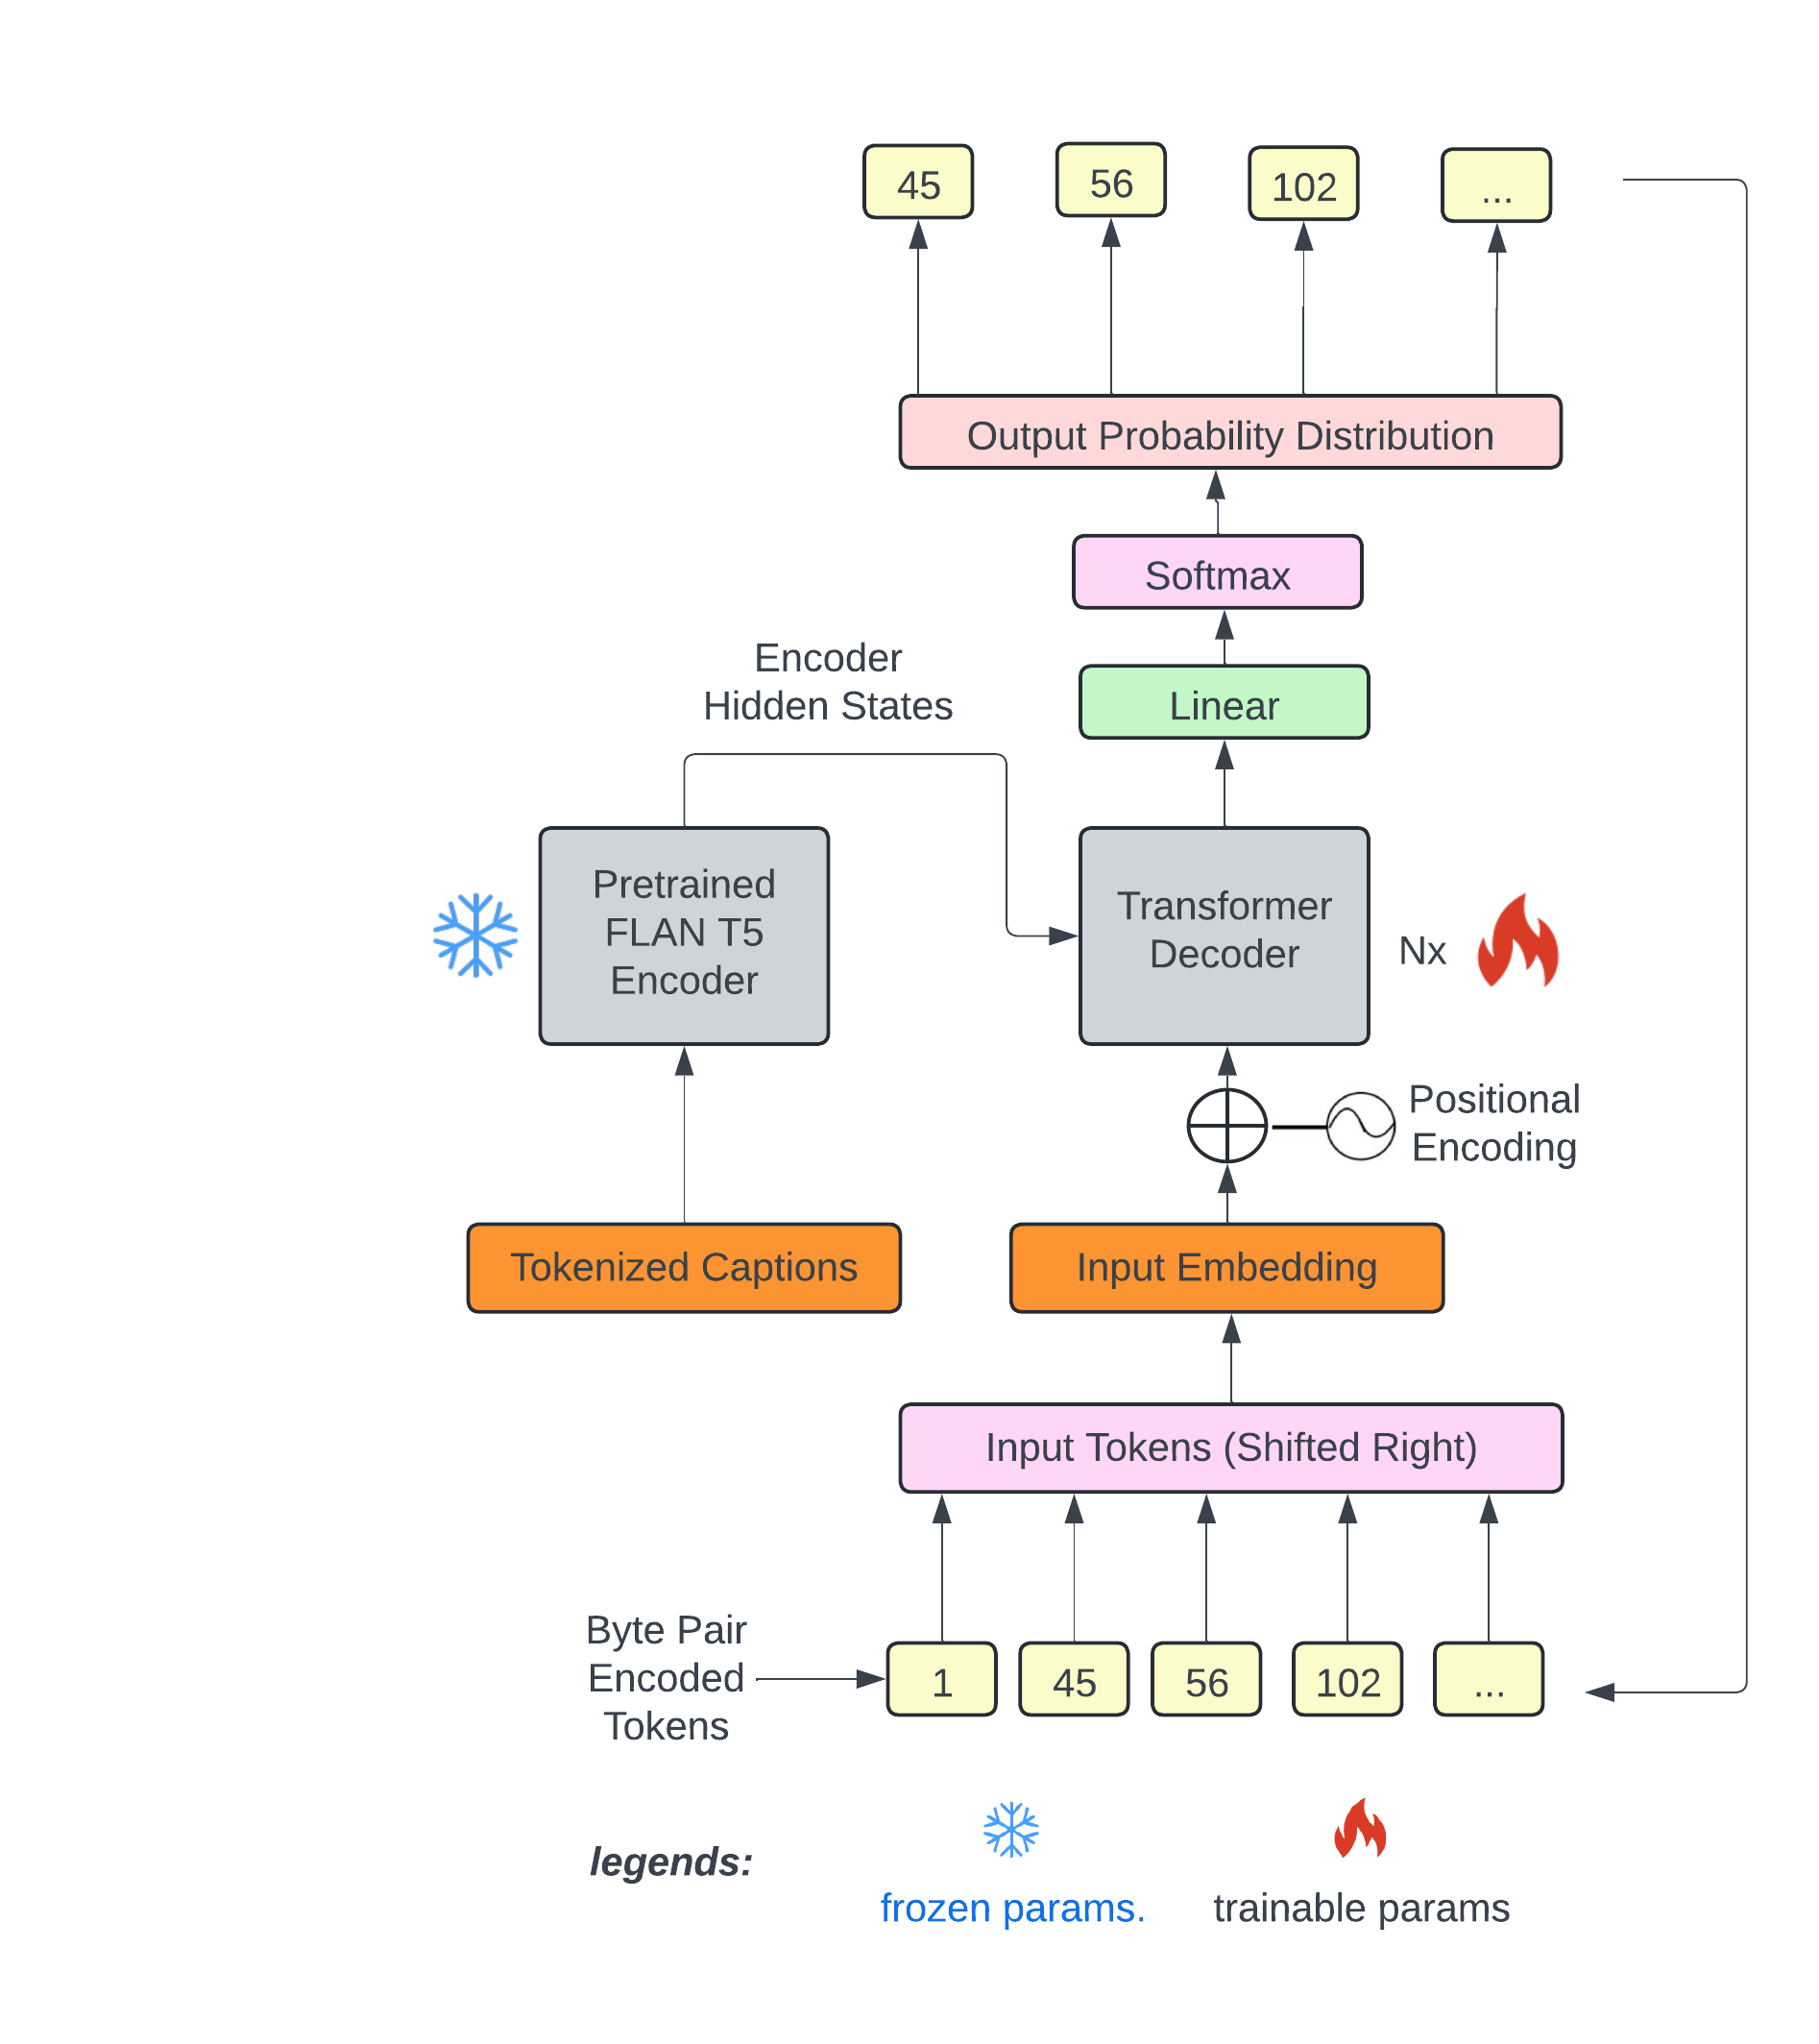
\includegraphics[width=0.48\textwidth]{figures/text2midi/text2midi_architecture.jpg}
\caption{Схема архитектуры Text2midi~\sourcecite{ref:bhandari2025text2midi}.}
\label{fig:text2midi-architecture}
\end{figure}

В дальнейшем модель трактуется как условная политика
$\pi_\theta(y \mid x)$, где $x$ --- текстовый запрос, а $y$ ---
сгенерированная MIDI-последовательность. Базовая модель уже умеет
порождать валидные MIDI, но может создавать лишние дорожки, слишком
плотные фрагменты, большое число ударных событий или материал, слабо
согласованный с текстовым запросом. Дообучение должно сместить распределение
ответов в сторону более предпочтительных кандидатов, не разрушая
исходную способность генерировать символьную музыку.

\subsection{GRPO как схема последующего дообучения}

Для последующего дообучения выбран \textit{Group Relative Policy
Optimization} (GRPO)~\sourcecite{ref:deepseekmath2024}. В text-to-MIDI эта схема
удобна по двум причинам: качество фрагмента оценивается после завершения
генерации, а один запрос допускает несколько музыкально корректных ответов.
GRPO не требует единственного эталона; вместо этого он сравнивает ответы
модели между собой и усиливает варианты с более высокой оценкой внутри
группы.

Пусть $q$ обозначает текстовый запрос, а $o_i$ --- $i$-ю
сгенерированную последовательность MIDI. На каждом шаге текущая политика,
зафиксированная на момент генерации, порождает группу из $G$ ответов:
\[
\{o_i\}_{i=1}^G \sim \pi_{\theta_{\mathrm{old}}}(O \mid q).
\]
Каждый ответ декодируется в MIDI и получает скалярную награду
$r_i = R(q,o_i)$. Награда вычисляется для всей последовательности:
её источником могут быть музыкальные правила, оценка внешнего критика
или их комбинация. Относительное преимущество ответа определяется
нормировкой наград внутри группы:
\[
\hat{A}_{i} =
\frac{r_i - \bar r}
{s_r+\varepsilon_A},
\qquad
\bar r = \frac{1}{G}\sum_{j=1}^{G} r_j,
\qquad
s_r = \operatorname{std}(r_1,\ldots,r_G).
\]
Так как награда относится к завершённому MIDI-фрагменту, одно и то же
значение $\hat{A}_{i}$ применяется ко всем токенам последовательности
$o_i$. Если в одном шаге используется несколько запросов, нормировка
выполняется отдельно для группы каждого запроса.

Для токена $o_{i,t}$ вводится отношение вероятностей новой и старой
политики:
\[
\rho_{i,t}(\theta)=
\frac{\pi_\theta(o_{i,t}\mid q,o_{i,<t})}
{\pi_{\theta_{\mathrm{old}}}(o_{i,t}\mid q,o_{i,<t})}.
\]
Отношение показывает, насколько обновляемая модель изменила
вероятность токена относительно политики, использованной при генерации
текущей группы. Для ограничения размера обновления применяется отсечение
по интервалу $[1-\epsilon,1+\epsilon]$. В реализации минимизируется
следующая функция потерь:
\[
\mathcal{L}_{\mathrm{GRPO}} =
\frac{1}{\sum_{i,t} m_{i,t}}
\sum_{i,t} m_{i,t}
\left(
-\min\big(
\rho_{i,t}(\theta)\hat{A}_{i},
\operatorname{clip}(\rho_{i,t}(\theta),1-\epsilon,1+\epsilon)\hat{A}_{i}
\big)
+\beta D_{i,t}
\right),
\]
где $m_{i,t}$ --- маска валидных токенов, $\epsilon$ задаёт допустимое
изменение политики за один шаг, а $\beta$ определяет вес регуляризации.
Слагаемое $D_{i,t}$ удерживает модель рядом с фиксированной опорной
моделью $\pi_{\mathrm{ref}}$:
\[
D_{i,t} =
\frac{\pi_{\mathrm{ref}}(o_{i,t}\mid q,o_{i,<t})}
{\pi_\theta(o_{i,t}\mid q,o_{i,<t})}
-
\log
\frac{\pi_{\mathrm{ref}}(o_{i,t}\mid q,o_{i,<t})}
{\pi_\theta(o_{i,t}\mid q,o_{i,<t})}
-1.
\]
На практике эта величина вычисляется через логарифмы вероятностей токенов.
Если ответ имеет положительное относительное преимущество, обновление
увеличивает вероятность составляющих его токенов; если преимущество
отрицательное, вероятность таких токенов уменьшается. KL-регуляризация
удерживает модель от слишком далёкого отклонения от
исходного генератора.

Особенности применения GRPO к text-to-MIDI приведены в
таблице \ref{tab:grpo_midi_specifics}.

\begin{table}[ht]
\centering
\caption{Особенности применения GRPO к задаче text-to-MIDI}
\label{tab:grpo_midi_specifics}
\begin{tabular}{|p{0.28\textwidth}|p{0.60\textwidth}|}
\hline
\textbf{Элемент} & \textbf{Реализация в работе} \\
\hline
Единица сравнения & Завершённая MIDI-последовательность, полученная после декодирования токенов. \\
\hline
Группа ответов & Несколько вариантов для одного текстового запроса; преимущества считаются внутри этой группы. \\
\hline
Награда & Скалярная оценка MIDI-фрагмента, вычисляемая правилами, критиком или их комбинацией. \\
\hline
Сигнал критика & В экспериментах используется сырая оценка критика, ранг внутри группы или доля попарных побед. \\
\hline
Ограничение обновления & Отсечение отношения вероятностей снижает риск резкого изменения политики. \\
\hline
Опорная модель & KL-слагаемое ограничивает отклонение от исходного генератора. \\
\hline
Валидность & Невалидные или вырожденные MIDI-фрагменты получают штраф и не должны усиливаться при обучении. \\
\hline
\end{tabular}
\end{table}

\subsection{Один шаг обучения в реализованной процедуре}

Процедура обучения строится вокруг одного итерационного шага GRPO.
На вход шага поступает один или несколько текстовых запросов.
В зависимости от конфигурации они могут выбираться из датасета,
генерироваться синтетически по шаблону или фиксироваться заранее для
диагностического эксперимента. Для каждого запроса модель генерирует
несколько независимых кандидатов с одинаковым текстовым
условием. Один шаг обучения поэтому содержит не отдельный ответ модели, а
группу вариантов для последующего сравнения.

Стадии одного шага сведены в таблицу \ref{tab:grpo_training_step}.
Ключевая особенность процедуры состоит в отложенной награде: качество
оценивается не во время выбора отдельного токена, а после декодирования всей
последовательности.

\begin{table}[ht]
\centering
\caption{Один шаг GRPO-дообучения в реализованной процедуре}
\label{tab:grpo_training_step}
\begin{tabular}{|p{0.08\textwidth}|p{0.24\textwidth}|p{0.54\textwidth}|}
\hline
\textbf{Этап} & \textbf{Операция} & \textbf{Назначение} \\
\hline
1 & Выбор запроса & Задаёт текстовое условие, для которого будет построена группа кандидатов. \\
\hline
2 & Генерация кандидатов & Модель порождает несколько MIDI-кандидатов при одном и том же условии. \\
\hline
3 & Декодирование & Токены преобразуются в музыкальное представление и MIDI-файл. \\
\hline
4 & Вычисление награды & Кандидат оценивается компонентами на основе правил или внешним критиком. \\
\hline
5 & Нормировка внутри группы & Награды превращаются в относительные преимущества кандидатов. \\
\hline
6 & Обновление GRPO & Обновляются обучаемые параметры с отсечением отношения вероятностей и KL-регуляризацией. \\
\hline
\end{tabular}
\end{table}

В реализации дополнительно сохраняются служебные артефакты каждого шага:
тексты запросов, MIDI-файлы сгенерированных кандидатов, значения
компонент награды, статистика валидности, контрольные точки модели и метрики обучения.
Такие артефакты нужны не только для воспроизводимости, но и для анализа
поведения модели. В задачах музыкальной генерации численная награда не всегда
полностью объясняет воспринимаемое качество, поэтому возможность
прослушать сохранённые MIDI и сопоставить их с компонентами награды
входит в экспериментальную процедуру.

\subsection{Настройка обучаемых параметров модели}

Полное обновление всех весов в режиме обучения с подкреплением дорого и
рискованно: награда шумна, а сильное изменение параметров может ухудшить
валидность MIDI. По этой причине используются ограниченные режимы настройки параметров
(таблица \ref{tab:adaptation_modes}).

\begin{table}[ht]
\centering
\caption{Режимы настройки обучаемых параметров}
\label{tab:adaptation_modes}
\begin{tabular}{|p{0.24\textwidth}|p{0.30\textwidth}|p{0.34\textwidth}|}
\hline
\textbf{Режим} & \textbf{Что обучается} & \textbf{Роль в экспериментах} \\
\hline
LoRA-адаптация~\sourcecite{ref:hu2021lora} & Низкоранговые добавки к выбранным линейным слоям & Основной экономичный режим для GRPO-дообучения. \\
\hline
Прямое частичное дообучение & Непосредственно выбранные параметры исходной модели & Более сильный, но потенциально менее устойчивый вариант. \\
\hline
\end{tabular}
\end{table}

На практике основным стал вариант LoRA только в FFN-блоках:
низкоранговые добавки подключаются к слоям декодера \texttt{linear1} и
\texttt{linear2}. Этот режим меняет распределение музыкальных токенов,
но оставляет большую часть модели замороженной. Прямое частичное
дообучение рассматривается как более сильный вариант, требующий меньшего
значения скорости обучения и более строгого контроля KL.

\subsection{Формирование текстовых запросов}

Текстовый запрос определяет группу кандидатов, внутри которой нормируются награды.
Он влияет не только на генерацию, но и на разброс обучающего
сигнала. В экспериментах используются короткие шаблонные запросы с
явно заданными атрибутами:
\[
\begin{aligned}
&\text{A moderate warm folk piece in C major at 96 BPM,}\\
&\text{with a 4/4 time signature. Use piano for the lead melody}\\
&\text{and acoustic guitar for steady accompaniment.}
\end{aligned}
\]

\subsection{Стратегия выбора запросов для обучения}

В экспериментах предусмотрены несколько режимов подачи текстовых запросов
(таблица \ref{tab:prompt_regimes}). Фиксированный запрос нужен для
диагностики обучаемости сигнала награды, а более широкие режимы --- для
проверки обобщения.

\begin{table}[ht]
\centering
\caption{Режимы формирования текстовых запросов в GRPO-экспериментах}
\label{tab:prompt_regimes}
\begin{tabular}{|p{0.23\textwidth}|p{0.32\textwidth}|p{0.33\textwidth}|}
\hline
\textbf{Режим} & \textbf{Что фиксируется} & \textbf{Зачем используется} \\
\hline
Фиксированный запрос & Все текстовые атрибуты постоянны & Диагностика обучаемости сигнала награды. \\
\hline
Случайные запросы & Атрибуты случайно выбираются из шаблона & Проверка обобщения на разные условия. \\
\hline
Учебная последовательность & Пространство запросов расширяется постепенно & Снижение шума и плавное усложнение задачи. \\
\hline
Смешанный режим & Часть запросов фиксирована, часть случайна & Совмещение диагностики и обобщения. \\
\hline
\end{tabular}
\end{table}

Дополнительно вводится учебная последовательность: сначала фиксируется простой
запрос, затем поэтапно меняются тональность, размер и стиль. Такой порядок
уменьшает разброс награды между шагами и помогает проверить, не
забывает ли модель уже освоенное поведение.

\subsection{Проектирование функции награды}

Функция награды подбиралась итеративно. Сначала проверялись
интерпретируемые MIDI-правила, затем критик v1 и критик v2, после этого
смешанные схемы. Подход согласуется с работами, где обучение с подкреплением
применяется к музыкальной генерации через внешние эстетические или
предпочтительные оценки~\sourcecite{ref:rlduet2020}, \sourcecite{ref:musicrl2024}, \sourcecite{ref:smart2025}.
Семейства сигналов награды приведены в таблице \ref{tab:reward_families}.

\begin{table}[ht]
\centering
\caption{Семейства функций награды}
\label{tab:reward_families}
\begin{tabular}{|p{0.22\textwidth}|p{0.34\textwidth}|p{0.32\textwidth}|}
\hline
\textbf{Семейство} & \textbf{Источник оценки} & \textbf{Роль в работе} \\
\hline
Символьные правила & Метрики, вычисляемые по MIDI-структуре & Контроль интерпретируемых музыкальных свойств. \\
\hline
Сигналы критика & Критик v1/v2 & Приближение более сложного музыкального предпочтения. \\
\hline
Смешанные схемы & Взвешенная комбинация правил и критика & Стабилизация оценки критика через простые ограничения. \\
\hline
\end{tabular}
\end{table}

\subsection{Структура используемых компонент награды}

\subsubsection{Общие обозначения и нормировка}

Все компоненты на основе правил вычисляются после декодирования токенов в
символьную MIDI-структуру. Обозначим множество нот через $N$, число нот
через $|N|$, длительность фрагмента в долях через $D$, число непустых
дорожек через $C$, долю барабанных нот через $\rho_d$, а текстовый
запрос через $x$. Для мягких ограничений используется треугольная
нормировка:
\[
T(z;l,c,h)=
\begin{cases}
0, & z\le l \ \text{или}\ z\ge h,\\
\dfrac{z-l}{c-l}, & l<z<c,\\
1, & z=c,\\
\dfrac{h-z}{h-c}, & c<z<h.
\end{cases}
\]
Эта функция задаёт целевой диапазон значений. Максимальная награда
достигается в точке $c$; отклонение в сторону слишком малых или слишком
больших значений линейно уменьшает вклад соответствующей компоненты.

\subsubsection{Тональная согласованность}

Компонента тональности использует длительно-взвешенный профиль высот
$p$ и сравнивает его с профилем тональности, заданной текстовым
запросом. Если $k_x$ --- целевой профиль, то
\[
a=\frac{\operatorname{corr}(p,k_x)+1}{2}, \qquad
b=\frac{\operatorname{corr}(p,k_x)-\max_{k\ne k_x}\operatorname{corr}(p,k)+1}{2},
\]
\[
R_{\mathrm{key}}=\operatorname{clip}(0.75a+0.25b,0,1).
\]
Первое слагаемое отражает абсолютное совпадение с целевой тональностью,
второе --- отделимость целевой тональности от альтернативных
тональностей.

\subsubsection{Метрическая организация}

Компонента метра оценивает не только записанный размер, но и
расположение акцентов в нотном материале. Для каждого кандидата
вычисляется соответствие $f_m$ нескольким метрическим шаблонам, после
чего целевой размер из текстового запроса получает оценку
\[
R_{\mathrm{meter}}=
\operatorname{clip}\!\left(0.7\frac{f_x}{\max_m f_m}+0.3f_x,0,1\right).
\]
Эта формула учитывает абсолютную выраженность целевого метра и его
относительное преимущество перед другими возможными размерами.

\subsubsection{Длительность и плотность нот}

Компоненты длительности и плотности также задаются через треугольную
нормировку:
\[
R_{\mathrm{dur}}=T(D;8,64,160), \qquad
R_{\mathrm{dens}}=T\!\left(\frac{|N|}{\max(D,1)};l,c,h\right).
\]
Компонента $R_{\mathrm{dur}}$ снижает награду для слишком коротких
фрагментов и чрезмерно длинных артефактов. Компонента
$R_{\mathrm{dens}}$ контролирует число нот на одну долю. Параметры
$l,c,h$ задаются в конфигурации эксперимента; так можно отдельно
исследовать обычную и умеренную плотность.

\subsubsection{Дорожки и ударные инструменты}

Аранжировочные ограничения задаются мягкими функциями. Компонента числа
дорожек поощряет непустые MIDI с числом дорожек не больше $C_{\max}$,
а при превышении лимита линейно убывает. Для ударных используется доля
барабанных нот:
\[
R_{\mathrm{drum}}=
\begin{cases}
1, & \rho_d\le a,\\
0, & \rho_d\ge b,\\
1-\dfrac{\rho_d-a}{b-a}, & a<\rho_d<b.
\end{cases}
\]
Такое правило не запрещает ударные полностью, но снижает награду, если
они начинают доминировать в MIDI-фрагменте.

\subsubsection{Валидность и внешний критик}

Проверка валидности служит защитным механизмом. Если MIDI не
декодируется, содержит слишком мало нот, слишком короткий фрагмент или
чрезмерное повторение одной высоты, выставляется индикатор
$I_{\mathrm{bad}}=1$. В экспериментах с внешним критиком дополнительно
вводится сигнал $R_{\mathrm{critic}}$: сырая оценка, ранг внутри
группы или доля попарных побед кандидата над другими вариантами.

\subsubsection{Итоговая функция награды}

Итоговая награда задаётся как взвешенная сумма активных компонент:
\[
R(x,y)=
\begin{cases}
-p_{\mathrm{bad}}, & I_{\mathrm{bad}}(y)=1 \ \text{и включён жёсткий фильтр},\\
\sum_k \lambda_k R_k(x,y)+\lambda_c R_{\mathrm{critic}}(x,y), & \text{иначе}.
\end{cases}
\]
Здесь $p_{\mathrm{bad}}$ --- штраф за невалидный MIDI, $\lambda_k$ ---
веса компонент на основе правил, а $\lambda_c$ --- вес внешнего критика. В
режиме обучения по критику ранговый сигнал особенно полезен тогда, когда
абсолютные значения критика плохо калиброваны, но порядок кандидатов
достаточно информативен.

\subsection{Конфликты между компонентами награды}

Добавление новых правил не всегда улучшает обучение: компоненты награды могут
конфликтовать. Это проверялось в пробных экспериментах с разными наборами
компонент: тональностью и метром, плотностью нот, ограничениями на дорожки,
запретом ударных и сигналами критика. После этих запусков часть бинарных
правил была заменена мягкими метриками, а веса наиболее жёстких компонент
были снижены. Выявленные конфликты приведены в таблице
\ref{tab:reward_conflicts}.

\begin{table}[ht]
\centering
\caption{Типичные конфликты между компонентами награды}
\label{tab:reward_conflicts}
\begin{tabular}{|p{0.25\textwidth}|p{0.33\textwidth}|p{0.30\textwidth}|}
\hline
\textbf{Конфликт} & \textbf{Причина} & \textbf{Практическое решение} \\
\hline
Плотность и естественность & Высокая плотность улучшает формальную заполненность, но может звучать перегруженно. & Переход к умеренной плотности. \\
\hline
Метр и свобода фразы & Шаблон метра помогает контролю, но может усиливать механичность. & Ослабление веса или временное отключение компоненты. \\
\hline
Запрет барабанов и обучаемость & Бинарный сигнал часто одинаков для всех кандидатов. & Замена на долю барабанных нот. \\
\hline
Число дорожек и полнота аранжировки & Жёсткое ограничение упрощает MIDI, но может удалить содержательные партии. & Мягкие ограничения и анализ сохранённых MIDI. \\
\hline
\end{tabular}
\end{table}

Состав функции награды уточнялся эмпирически: анализировались не только
суммарный сигнал и вклад отдельных компонент, но и сохранённые MIDI-примеры.

\subsection{Ожидаемые преимущества и исследовательские гипотезы}

Гипотезы работы сведены в таблицу \ref{tab:approach_hypotheses}.

\begin{table}[ht]
\centering
\caption{Ожидаемые эффекты предлагаемого подхода}
\label{tab:approach_hypotheses}
\begin{tabular}{|p{0.30\textwidth}|p{0.58\textwidth}|}
\hline
\textbf{Гипотеза} & \textbf{Ожидаемый эффект} \\
\hline
GRPO применим к text-to-midi & Модель сможет усиливать более удачные MIDI-кандидаты без эталонной последовательности. \\
\hline
Ограниченная настройка параметров достаточна & LoRA или частичное дообучение смогут изменить поведение модели без полного обновления всех весов. \\
\hline
Мягкие компоненты награды лучше бинарных & Непрерывные сигналы будут чаще различать кандидатов внутри группы. \\
\hline
Узкое распределение запросов снижает шум & Фиксированный запрос и учебная последовательность позволят яснее увидеть динамику обучения. \\
\hline
Внешний критик может служить источником награды & Сигнал критика позволит согласовывать модель с более сложными критериями качества. \\
\hline
\end{tabular}
\end{table}

\chapter{Экспериментальная часть}

\subsection{Цели экспериментального исследования}

Экспериментальная часть проверяет, можно ли использовать предложенную схему
для последующего дообучения text-to-MIDI модели. В отличие от стандартного
обучения с эталонной MIDI-последовательностью, здесь модель получает только
текстовый запрос и несколько собственных вариантов ответа. Главный вопрос
состоит в том, достаточно ли относительных оценок MIDI-кандидатов для
устойчивого обновления модели.

Первая цель --- проверить саму возможность дообучения с подкреплением
для символьной музыкальной генерации. Необходимо установить, приводит ли
обновление параметров по групповым оценкам к изменению поведения модели,
не разрушая при этом способность генерировать валидные MIDI-файлы. Для
этого анализируются значения итоговой награды, доля
валидных генераций, характер ошибок декодирования, динамика KL-штрафа и
изменение отдельных компонент награды.

Вторая цель --- сравнить источники награды: интерпретируемые правила,
критик v1/v2 и смешанные схемы. Компоненты на основе правил
контролируют простые
музыкальные свойства: тональность, метр, длительность, плотность нот и
долю ударных событий. Критик, напротив, должен приближать более сложное
предпочтение, которое трудно выразить набором простых формул. В этих
экспериментах проверяется, какие сигналы дают различимые оценки
внутри группы кандидатов и какие из них приводят к более устойчивому
обновлению модели.

Третья цель --- выбрать режим адаптации параметров. Полное дообучение модели
в режиме обучения с подкреплением вычислительно дорого и может приводить к
нестабильным изменениям политики. Сравнение ведётся между более ограниченными
режимами: LoRA-адаптацией выбранных слоёв, настройкой FFN-блоков и частичным
дообучением. Здесь важен не только рост награды, но и устойчивость обучения:
отсутствие резких скачков функции потерь, чрезмерного роста KL и деградации
качества MIDI.

Ещё одна задача --- сопоставить внутренние метрики обучения с внешней оценкой
качества. Рост суммарной награды сам по себе
не гарантирует улучшения музыкального результата: модель может
переоптимизироваться под отдельную компоненту, например чрезмерно
увеличить плотность нот или механически следовать метрическому шаблону.
Итоговая оценка строится не только по логам обучения, но и по
построенному A/B-сравнению базовой и дообученной модели, а также по
оценкам внешней модели-оценщика.

\subsection{Инфраструктура и программная реализация}

Экспериментальная инфраструктура реализована как расширение открытого проекта
Text2MIDI\footnote{blank}. В кодовую базу добавлены процедура последующего
GRPO-дообучения, модуль вычисления наград, система конфигураций и средства
сохранения результатов. Реализация организована модульно: отдельно задаются
конфигурации запусков, процедура обучения, компоненты функции награды и
инструменты последующего анализа.

Программная часть написана на языке Python~\sourcecite{ref:python2026}, а
обучение нейросетевых моделей и вычисление градиентов выполняются с
использованием PyTorch~\sourcecite{ref:pytorch2019}. Этот стек даёт возможность гибко
управлять генерацией последовательностей, повторно
вычислять логарифмы вероятностей токенов для GRPO и сохранять состояние
оптимизатора между запусками.

Обучение запускается по имени эксперимента. Для каждого запуска
создаётся YAML-конфигурация, в которой фиксируются параметры GRPO:
число текстовых запросов на шаг, число генерируемых кандидатов,
максимальная длина генерации, скорость обучения, веса компонент награды и
режим адаптации параметров модели. Часть параметров можно переопределить
из командной строки; это упрощает проведение серий
сопоставимых экспериментов.

Во время обучения сохраняются контрольные точки модели, значения
отдельных компонент награды, служебные метрики оптимизации и,
при необходимости, промежуточные MIDI-кандидаты. Логирование ведётся в
Weights \& Biases~\sourcecite{ref:wandb2026}: по этим логам сопоставляются динамика суммарной награды
с поведением отдельных компонент, KL-штрафом, функцией потерь, нормами градиентов
и статистикой валидности. Логи запусков и связанные с ними артефакты
экспериментов доступны в материалах репозитория.

\subsection{Семейства исследуемых конфигураций}

Эксперименты организованы как несколько семейств конфигураций, а не как один
длинный запуск. Такое разделение помогает отдельно оценить влияние источника
награды, длины генерации, способа выбора текстовых запросов и набора обучаемых
параметров. Базовая модель во всех случаях остаётся одной и той же, а различия
между запусками задаются через конфигурационные файлы.

Первое семейство составляют запуски с наградами на основе явно заданных
музыкальных правил. В них модель получает сигнал за соответствие тональности,
метрической структуре, умеренной плотности нот, балансу длительности и
ограничению доли ударных событий. Эти эксперименты показывают, может ли GRPO
улучшать формальные свойства MIDI без привлечения обученного музыкального
критика.

Во втором семействе основной наградой служит только критик выбранной версии.
В таких запусках качество не задаётся вручную в виде отдельных
компонент; модель получает скалярный сигнал, полученный из ранжирования
нескольких сгенерированных вариантов. Здесь проверяется, достаточно ли
обобщённого сигнала качества для устойчивого дообучения генератора.

Третье семейство объединяет оба подхода: часть награды задаётся правилами, а
часть --- критиком. Такие конфигурации рассматриваются как компромисс между
интерпретируемостью ручных признаков и более общей оценкой музыкальности.
Предварительные запуски показали, что слишком большое число одновременно
активных компонент может давать конфликтующие градиенты; поэтому смешанные
конфигурации проверялись в нескольких вариантах с разными весами.

Также рассматривались эксперименты с отбором дорожек после генерации.
В них из исходного MIDI выбирались наиболее информативные неударные дорожки,
после чего уже этот вариант передавался в вычисление награды. Эти запуски
отделяют качество музыкального материала от шума, возникающего из-за
пустых, слишком коротких или преимущественно ударных дорожек. Позднее
проверялись и конфигурации без такого отбора, чтобы оценить, способна ли
модель научиться генерировать более подходящую структуру напрямую.

Ещё одна группа экспериментов связана с ограничением пространства текстовых
запросов. Вместо немедленного обучения на широком наборе
описаний использовались фиксированный запрос и небольшой учебный набор,
в котором постепенно менялись тональность, размер и стиль. Учебная
последовательность нужна для диагностики: если модель не демонстрирует
изменений даже на узком классе запросов, то расширение набора описаний не
устраняет проблему, а лишь увеличивает шум оценки.

\begin{table}[h]
\centering
\caption{Основные семейства экспериментальных конфигураций}
\label{tab:experiment-families}
\begin{tabular}{|p{0.25\textwidth}|p{0.33\textwidth}|p{0.32\textwidth}|}
\hline
\textbf{Семейство} & \textbf{Основная идея} & \textbf{Что проверяется} \\
\hline
Правила & Награда из музыкальных признаков: тональность, метр, плотность,
длительность, доля ударных & Способность GRPO улучшать явно заданные
свойства MIDI \\
\hline
Критик v1/v2 & Награда строится по ранжированию сгенерированных вариантов &
Достаточность обученного сигнала качества без ручных правил \\
\hline
Правила + критик v1/v2 & Сумма интерпретируемых компонент и оценки критика &
Баланс между устойчивостью правил и обобщённой музыкальной оценкой \\
\hline
Отбор дорожек & Награда считается после выбора информативных неударных
дорожек & Влияние пустых и шумовых дорожек на обучение \\
\hline
Учебная последовательность запросов & Постепенное усложнение: базовое
описание, тональность, размер, стиль & Возможность увидеть эффект обучения
на узком и контролируемом наборе условий \\
\hline
\end{tabular}
\end{table}

\subsection{Конфигурации текстовых запросов и режимов генерации}

В GRPO один шаг обучения строится не по отдельной сгенерированной
последовательности, а по группе кандидатов для одного или нескольких
текстовых описаний. Если на шаге используется $P$ описаний и для каждого
описания генерируется $G$ вариантов, то всего на шаг получается
$P \cdot G$ MIDI-кандидатов. Награды нормируются внутри группы вариантов,
относящихся к одному и тому же описанию, поэтому выбор $P$ и $G$ напрямую
влияет на шумность обучающего сигнала.

В начальных экспериментах использовались более широкие наборы описаний:
несколько запросов на шаг и небольшое число кандидатов для каждого
из них. Этот режим быстрее покрывает разные музыкальные условия, но
увеличивает разброс наград: модель одновременно видит разные тональности,
размеры, стили и требования к фактуре. Для ранней проверки работоспособности
алгоритма это полезно, однако по таким кривым сложнее понять, действительно
ли модель подстраивается под награду или изменения объясняются случайностью
генерации.

В последующих диагностических запусках пространство запросов было
сужено. Главный диагностический режим --- один запрос на шаг и увеличенное число
кандидатов. Например, в конфигурациях с 18 вариантами на один запрос один
шаг обучения содержит 18 MIDI-кандидатов, а в запусках с критиком ---
25 кандидатов. Это делает относительное сравнение
внутри группы более устойчивым: все варианты отвечают одному и тому же
текстовому условию, а различия в награде сильнее связаны с качеством самой
генерации.

Максимальная длина генерации задаёт верхнюю границу числа генерируемых
токенов. Для быстрых диагностических экспериментов использовалась длина 800:
она даёт достаточно содержательный музыкальный фрагмент, но
не делает генерацию чрезмерно дорогой. Проверялись и более длинные
варианты, однако увеличение длины заметно повышает время одного шага и может
усиливать шум награды, если модель начинает генерировать слишком плотный или
неустойчивый материал.

Параметр \texttt{generation\_chunk\_size} отвечает только за техническое
разбиение генерации на части. Он не меняет число кандидатов в GRPO-группе, но
помогает подстроить запуск под доступную видеопамять. Параметр
\texttt{update\_mini\_batch} аналогично задаёт размер части кандидатов,
используемой при вычислении обновления. В основных диагностических запусках
оба параметра выбирались равными числу кандидатов, чтобы весь набор
вариантов для одного запроса обрабатывался без дополнительного дробления.

Для проверки способности модели удерживать простые изменения условий была
добавлена учебная последовательность запросов. Она состоит из четырёх
этапов: сначала фиксируется базовое описание, затем меняется тональность,
после этого размер, а на последнем этапе --- стиль. При переходе к новым
этапам часть ранних запросов повторяется, чтобы уменьшить забывание уже
освоенных условий. Этот режим не предназначен для финальной оценки качества
на широком наборе описаний; его задача --- показать, появляется ли управляемое
изменение поведения модели в простой и контролируемой постановке.

\subsection{Сравниваемые стратегии адаптации параметров}

Исходная Text2MIDI-модель уже обучена генерировать MIDI, поэтому полное
переобучение всех параметров не проводится. Вместо этого сравниваются
ограниченные режимы настройки, в которых изменяется только небольшая часть
модели. Такой выбор снижает вычислительные требования и уменьшает риск разрушить уже
выученную способность генерировать синтаксически корректные
MIDI-последовательности.

Главный режим основан на LoRA~\sourcecite{ref:hu2021lora}: веса исходной модели
замораживаются, а к выбранным линейным преобразованиям добавляются обучаемые
низкоранговые матрицы. В экспериментах проверялись три варианта такого
подключения. Первый вариант изменяет только слои внимания
(\texttt{to\_qkv}, \texttt{to\_out}); он потенциально влияет на связи между
токенами и структуру последовательности. Второй вариант изменяет только
FFN-блоки декодера (\texttt{linear1}, \texttt{linear2}); он оказался
более удобным для локального смещения распределения музыкальных токенов без
резкой перестройки внимания. Третий вариант объединяет оба набора слоёв и
даёт модели больше свободы, но требует более осторожного выбора скорости
обучения и KL-ограничения.

Также рассматривалось прямое частичное дообучение. В этом режиме
LoRA-добавки не используются: выбранные параметры самой модели становятся
обучаемыми, а остальные веса остаются замороженными. Этот вариант сильнее
воздействует на модель, из-за чего для него применялись меньшие значения скорости обучения и
более строгий контроль KL. На практике он полезен как проверка того, не
ограничивает ли LoRA слишком сильно пространство возможных изменений.

\begin{table}[h]
\centering
\caption{Сравниваемые режимы настройки параметров}
\label{tab:adaptation-strategies}
\begin{tabular}{|p{0.24\textwidth}|p{0.32\textwidth}|p{0.34\textwidth}|}
\hline
\textbf{Режим} & \textbf{Обучаемые параметры} & \textbf{Назначение в экспериментах} \\
\hline
LoRA на слоях внимания & \texttt{to\_qkv}, \texttt{to\_out} &
Проверка влияния на зависимости между токенами и организацию последовательности \\
\hline
LoRA на FFN & \texttt{linear1}, \texttt{linear2} &
Основной устойчивый режим для поздних запусков с правилами и критиком \\
\hline
LoRA на слоях внимания и FFN & Все перечисленные выше слои &
Более гибкая, но менее стабильная настройка распределения генерации \\
\hline
Прямое частичное дообучение & Выбранные параметры исходной модели &
Проверка более сильного вмешательства при меньшей скорости обучения \\
\hline
\end{tabular}
\end{table}

Для итоговых серий наиболее важным оказался режим LoRA на FFN-блоках. Он
сохраняет базовую структуру генератора и при этом заметно меняет
вероятности локальных музыкальных решений: выбор длительностей, плотность нот,
распределение инструментальных событий и реакцию на сигнал критика. В итоге
этот режим использовался в учебных последовательностях запросов и в
поздних экспериментах с фиксированным запросом.

\subsection{Внутренние метрики и диагностика обучения}

Во время обучения фиксируются итоговая награда и значения отдельных
компонент. По ним можно понять, за счёт чего меняется поведение модели:
например, растёт ли награда из-за лучшего соответствия тональности, из-за
снижения доли ударных событий или из-за сигнала обученного критика. Для
смешанных функций награды такой разбор особенно важен, поскольку рост одной
компоненты может сопровождаться ухудшением другой.

Также отслеживаются служебные метрики оптимизации: функция потерь, величина
KL-расхождения с исходной политикой, норма градиента и отношение вероятностей
новой и старой политики. Эти величины используются как признаки устойчивости
обучения. Например, резкий рост KL показывает, что модель слишком далеко
отходит от исходного распределения, а большие скачки нормы градиента могут
указывать на слишком высокую скорость обучения или слишком шумную награду.

Также учитываются показатели валидности MIDI-последовательностей и частота
пропущенных обновлений, если соответствующая проверка включена в конфигурации.
Они помогают отделить настоящий рост качества от ситуаций, когда модель
получает высокую награду на технически неудачных или плохо декодируемых
последовательностях.

Внутренние метрики не рассматриваются как окончательная оценка музыкального
качества. Они показывают ход оптимизации, но не гарантируют, что результат
стал лучше на слух. Вместе с ними проводится внешнее сравнение
с базовой моделью.

\subsection{Построение внешней оценки качества}

Итоговая проверка качества проводится отдельно от процесса обучения. Награда
участвует в обновлении модели и сама по себе не является независимым
критерием. После завершения выбранного запуска сравниваются генерации базовой
модели и дообученной версии на одном и том же наборе текстовых запросов.

Для каждого запроса генерируется несколько MIDI-вариантов от обеих моделей.
Результаты агрегируются двумя способами: по среднему качеству нескольких
генераций и по лучшему варианту из группы. Первый показатель отражает
стабильность модели, второй --- её способность хотя бы иногда выдавать сильный
пример.

\subsubsection{A/B-сравнение базовой и дообученной модели}

В A/B-сравнении для каждого запроса определяется, какая из двух моделей
получила более высокую агрегированную оценку. Затем считается число побед
базовой и дообученной модели, доля побед и статистическая значимость по
знаковому критерию. Эта схема не требует сравнивать
абсолютные значения награды для разных запросов напрямую.

\subsubsection{Оценка с помощью внешней языковой модели}

Для дополнительной проверки MIDI переводится в ABC-нотацию~\sourcecite{ref:abcnotation2026}. Это
представление сохраняет тональность, размер, голоса и последовательность нот,
но остаётся текстовым и подходит для передачи в языковую модель. В роли
оценщика использовалась модель DeepSeek~\sourcecite{ref:deepseekv3report2024}: ей передавались текстовый запрос и
ABC-запись сгенерированного MIDI, после чего возвращались численная оценка и
краткое объяснение.

Сравнение также проводится в формате A/B-теста. Для одного и того же запроса
сопоставляются оценки генераций базовой и дообученной модели, затем
агрегируются победы по запросам. Эта оценка не используется как награда во
время обучения; она нужна для независимой проверки того, совпадает ли рост
внутренних метрик с внешней музыкальной оценкой.

\chapter{Результаты экспериментов}

В этот раздел выносятся численные результаты и графики после завершения
финальных запусков. Сначала приводится динамика обучения, затем сравнение
моделей и внешняя оценка качества.

\subsection{Динамика обучения}

На первом этапе проверялось, способен ли предложенный контур GRPO-дообучения
изменять поведение text-to-midi модели по завершённому MIDI-фрагменту, а не
только по токенам. Для этого рассматривались запуски с интерпретируемыми
наградами, учебной последовательностью prompt-ов и последующим подключением
критика. Динамика обучения показывает, что модель действительно реагирует на
внешний сигнал: отдельные компоненты награды начинают изменяться в ожидаемом
направлении, а лучшие кандидаты в группе становятся качественнее по заданным
критериям.

\begin{figure}[H]
\centering
\includegraphics[width=0.88\textwidth]{graphics/figures/wandb/01_fixed_prompt_rule_components_step15.pdf}
\caption{Динамика компонент награды при обучении по правилам на узком наборе текстовых запросов.}
\label{fig:fixed-prompt-rule-components}
\end{figure}

На рис.~\ref{fig:fixed-prompt-rule-components} показан начальный участок
обучения модели на узком наборе текстовых запросов. Уже в этом простом режиме
видно, что модель подстраивается под награды, заданные на уровне MIDI:
усиливается соответствие тональности, снижается доля нежелательных ударных
событий, а суммарная награда растёт относительно первых итераций. Такой
результат важен как техническая проверка всей схемы: награда вычисляется после
декодирования MIDI, но всё равно создаёт обучающий сигнал для языковой модели.
Более шумная компонента плотности нот показывает, что не все музыкальные
свойства одинаково легко оптимизируются простыми правилами.

\begin{figure}[H]
\centering
\includegraphics[width=0.88\textwidth]{figures/wandb/02_curriculum_reward_total_presentation.pdf}
\caption{Динамика общей награды при поэтапном обучении. Бледная линия показывает фактические значения, синяя --- сглаженную динамику, оранжевая --- лучшее достигнутое значение.}
\label{fig:curriculum-reward-total}
\end{figure}

На рис.~\ref{fig:curriculum-reward-total} показан запуск с учебной
последовательностью запросов. Вертикальные линии отделяют этапы, на которых
изменялись тональность, метрическая структура и стиль. По сравнению с
немедленным обучением на разнородных prompt-ах такая схема оказалась более
удобной для анализа: модель сначала закрепляет поведение на простом запросе, а
затем переносит его на близкие варианты.

\begin{figure}[H]
\centering
\includegraphics[width=0.88\textwidth]{figures/wandb/04_critic_top1_raw_after40_to_peak.pdf}
\caption{Дообучение по критику v2 после предварительного обучения на правилах. Синяя линия соответствует фактическим значениям, оранжевая --- лучшему достигнутому значению.}
\label{fig:critic-after-curriculum-top1}
\end{figure}

На рис.~\ref{fig:critic-after-curriculum-top1} отдельно показан этап, где
модель продолжает обучение уже по сигналу критика v2. Предварительное обучение на
правилах здесь играет роль стабилизации: критик v2 подключается не к полностью
исходной модели, а к модели, которая уже частично соблюдает простые музыкальные
ограничения. В этом режиме удаётся получить отдельные кандидаты с заметно более
высокой оценкой критика v2, что подтверждает полезность последовательной схемы
``правила затем критик v2''. При этом сам сигнал критика v2 остаётся более шумным,
чем ручные правила; это ограничение подробнее обсуждается в разделе анализа
ошибок.

\begin{figure}[H]
\centering
\includegraphics[width=0.88\textwidth]{figures/wandb/08_broad_prompt_first_critic_orange.pdf}
\caption{Обучение с критиком v1 на случайных prompt-ах. Показан запуск, в котором широкое распределение запросов привело к неустойчивой динамике общей награды.}
\label{fig:broad-prompt-first-critic}
\end{figure}

Рис.~\ref{fig:broad-prompt-first-critic} приведён как контрольный пример:
слишком широкое распределение запросов затрудняет обучение и делает награду
менее интерпретируемой. Этот результат полезен методически, поскольку
показывает, почему дальнейшие эксперименты были сосредоточены на узком наборе текстовых запросов и учебной последовательности, а не на случайном смешивании большого
числа условий.

\begin{figure}[H]
\centering
\includegraphics[width=0.88\textwidth]{figures/wandb/10_critic_v2_low_lr_top1_raw_step12.pdf}
\caption{Обучение с критиком v1 и уменьшенным шагом обучения.}
\label{fig:critic-v2-low-lr-step12}
\end{figure}

На рис.~\ref{fig:critic-v2-low-lr-step12} показан запуск дообучения модели на критике v1 на уменьшенном шаге обучения и узком наборе текстовых запросов.

\subsection{A/B-сравнение}

Для внутреннего сравнения использовались те же MIDI-файлы, что и для
последующей внешней оценки: по 900 генераций на модель при одинаковых условиях
текстового запроса. Для каждой дообученной модели использовался только тот источник
оценки, по которому она обучалась: модели с правилами сравнивались по
суммарной награде на основе правил, а модели с критиком --- по оценке
соответствующего критика.
Такое сравнение не смешивает разные цели оптимизации и показывает, улучшилась
ли модель именно относительно собственного обучающего сигнала.

На рис.~\ref{fig:ab-comparison-results} показана доля попарных побед
дообученной модели над базовой; значение 0.5 соответствует паритету.

\begin{figure}[H]
\centering
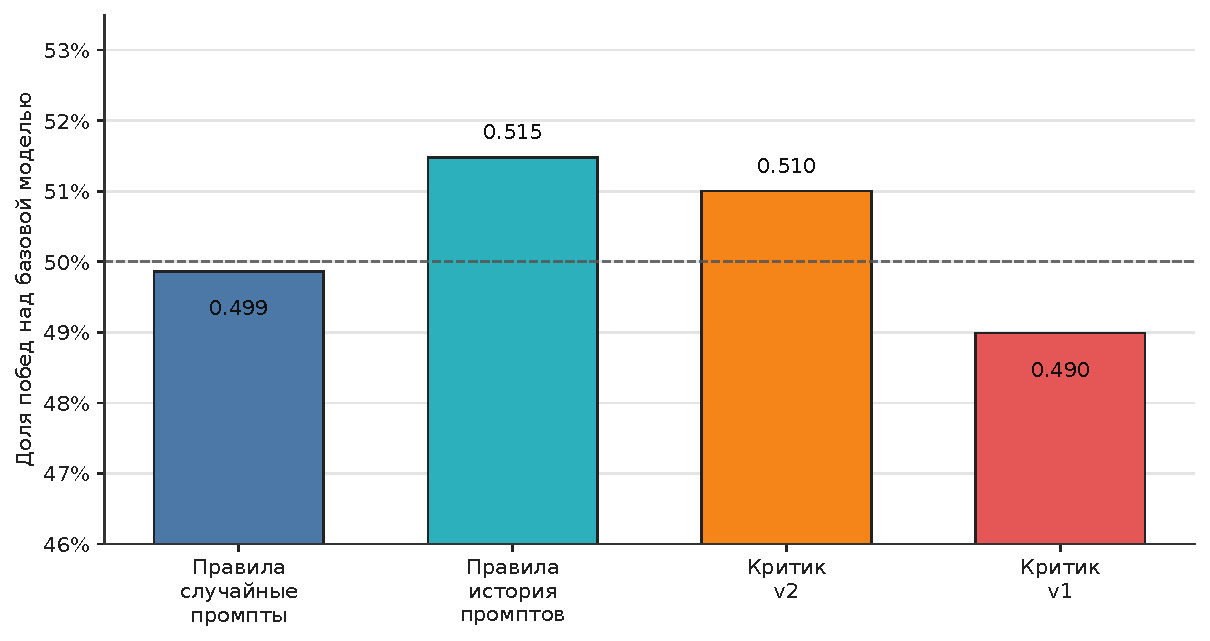
\includegraphics[width=0.95\textwidth]{figures/fixed_prompt_ab/reward_ab_own_metric.pdf}
\caption{A/B-сравнение с базовой моделью по собственному источнику награды. Показана доля попарных побед над базовой моделью.}
\label{fig:ab-comparison-results}
\end{figure}

\subsection{Оценка внешней языковой моделью}

Дополнительно была проведена пилотная оценка внешней языковой моделью
DeepSeek v3.2 через API AITunnel. Сравнивались две модели: базовая
text-to-midi модель и модель, дообученная по схеме ``правила затем критик
v2''. MIDI-файлы предварительно переводились в ABC, после чего в DeepSeek
передавался оценочный prompt. В нём модель задавалась как эксперт по
символьной музыке и получала инструкцию оценить качество связи мелодии и
гармонии: соответствие мелодических нот активным аккордам и тональности,
поддержку сильных долей, оправданность диссонансов и хроматизмов,
согласованность смены аккордов с ритмом мелодии, а также естественность
басового движения. Отдельно указывалось игнорировать качество тембров,
сведения, реалистичность инструментов и другие артефакты MIDI-производства.
Ответ требовался в формате \texttt{Score: <1-10>} и короткого объяснения.
Если численная оценка не была извлечена из ответа модели, значение считалось
равным 0.

\begin{table}[h]
\centering
\caption{Пилотная внешняя оценка DeepSeek v3.2}
\label{tab:external-score-results}
\begin{tabular}{|p{0.34\textwidth}|p{0.16\textwidth}|p{0.16\textwidth}|p{0.22\textwidth}|}
\hline
\textbf{Модель} & \textbf{Средняя оценка} & \textbf{Медиана} & \textbf{Максимальная оценка} \\
\hline
Базовая модель & 1.90 & 2.00 & 6.00 \\
\hline
Критик v1 после правил & 2.80 & 2.00 & 9.00 \\
\hline
\end{tabular}
\end{table}

По средней оценке дообученная модель превосходит базовую на 0.90 балла. Этот
результат следует рассматривать как предварительный: объём внешней оценки
мал, а отдельные ответы языковой модели могут быть нестабильны. Тем не менее
он согласуется с основной гипотезой эксперимента: предварительное обучение на
простых правилах может подготовить модель к последующему использованию более
сложного сигнала критика.

\chapter{Анализ ошибок и ограничений}

Несмотря на положительные диагностические результаты, эксперименты выявили
ряд ограничений, которые мешают получить устойчивую и крупную победу над
базовой моделью. Эти ограничения важны, потому что они показывают не только
слабые места конкретных запусков, но и требования к дальнейшему развитию
метода.

Первая проблема связана с плотностью нот. Простое поощрение заполненности
может быстро привести к переоптимизации: модель начинает генерировать слишком
быстрые и перегруженные фрагменты. Формально такие примеры получают высокую
оценку по компоненте плотности, но при прослушивании звучат менее естественно.
Это показывает, что музыкальная ``насыщенность'' не сводится к числу нот.
Поэтому в поздних конфигурациях максимизация плотности была заменена более
осторожной наградой за умеренный диапазон значений.

Вторая проблема связана с ударными и пустыми дорожками. Базовая модель часто
создаёт дополнительные дорожки, которые либо почти не содержат нот, либо
состоят преимущественно из ударных событий. Это искажает как награду, так и
восприятие результата: MIDI может выглядеть насыщенным, хотя содержательная
мелодико-гармоническая часть остаётся слабой. Режимы с отбором информативных
неударных дорожек частично решают задачу, но одновременно вносят ещё один
эвристический слой в обработку результата.

Наиболее существенное ограничение связано с критиком. Он предполагает, что
MIDI можно представить как две музыкальные роли: ведущую мелодию и
гармоническое сопровождение. Перед оценкой выполнялась проекция исходного MIDI
в формат \texttt{melody}/\texttt{chords}: сначала выбиралась наиболее
мелодическая неударная дорожка по эвристикам высоты, полифонии и поступенного
движения, а остальные неударные дорожки объединялись в сопровождение. Если
такой вариант давал слишком мало материала, использовалась резервная проекция
по событиям, где верхний голос считался мелодией, а остальные ноты ---
сопровождением.

Такая проекция делает вход критика совместимым с его обучающим форматом, но
добавляет шум. Ошибка выбора мелодической дорожки, потеря многоголосной
фактуры или неудачное разделение верхнего голоса и аккордовых нот могут
изменить оценку независимо от реального качества MIDI. Поэтому запуски только
с критиком нельзя трактовать как чистое измерение музыкального качества: они
оценивают связку из модели, процедуры проекции и самого критика.

Отдельным недостатком оказалась чувствительность к пространству текстовых
запросов. При слишком широком наборе описаний на ранних этапах обучение
становится плохо интерпретируемым: модель одновременно получает сигналы по
разным тональностям, размерам, стилям и фактурам. В таких условиях суммарная
награда не демонстрирует устойчивого роста, а отдельные удачные пики могут
быть следствием случайной генерации. Именно поэтому диагностические запуски с
одним фиксированным запросом и учебная последовательность оказались более
информативными.

Наконец, сохраняется высокая вычислительная стоимость экспериментов.
Увеличение максимальной длины генерации даёт потенциально более полный
музыкальный фрагмент, но существенно замедляет шаг обучения и может усиливать
проблемы с плотностью нот. Длина 800 токенов использовалась как практический
компромисс между скоростью диагностики и содержательностью результата, однако
для финальной оценки музыкальности требуется проверка и на более длинных
фрагментах.
\newpage
\chapter{Заключение}

В работе была исследована схема последующего дообучения text-to-MIDI модели
по внешним критериям качества. В отличие от обычного контролируемого
дообучения, где модель оптимизирует предсказание следующего токена,
использованный подход оценивает уже завершённые MIDI-фрагменты. Это позволило
работать с теми свойствами, которые проявляются на уровне целой музыкальной
последовательности: тональной согласованностью, ритмической устойчивостью,
плотностью фактуры, долей ударных событий и общей структурной связностью.

В ходе работы был реализован полный цикл GRPO-дообучения: генерация группы
кандидатов для текстового запроса, декодирование MIDI, вычисление награды,
обновление LoRA-параметров и последующая диагностика качества. Были
исследованы два типа обучающего сигнала. Первый основан на интерпретируемых
правилах и позволяет контролировать отдельные свойства MIDI. Второй использует
графовый критик, оценивающий музыкально-теоретическую согласованность
фрагмента через отношения между мелодией, гармонией и метрической структурой.

Положительным результатом стало то, что в диагностических режимах модель
реагировала на выбранный источник награды: rule-based конфигурации улучшали
часть формальных музыкальных признаков, а использование более сильного
критика после предварительного обучения на правилах дало более благоприятный
результат в сравнении с базовой моделью. Это подтверждает основную гипотезу
работы: последующее дообучение может смещать распределение генераций в сторону
кандидатов, предпочтительных по заданному музыкальному критерию.

В то же время эксперименты показали ограничения подхода. Простые правила
могут конфликтовать между собой: например, поощрение плотности нот без
дополнительных ограничений приводит к чрезмерно насыщенной фактуре. Качество
критика также существенно влияет на результат: слабый или смещённый критик
может поощрять формальные признаки, не совпадающие с воспринимаемой
музыкальностью. Кроме того, проекция произвольного MIDI в представление
мелодии и аккомпанемента добавляет шум, поэтому итоговая оценка зависит не
только от сгенерированного фрагмента, но и от процедуры его структурного
разбора.

Дальнейшее развитие работы прежде всего требует более надёжной внешней
проверки музыкального качества. Помимо автоматических оценок, нужен
зрительский тест: слушателям можно предъявлять пары MIDI или аудиорендеров,
полученных базовой и дообученной моделью, и просить выбрать более музыкальный,
согласованный с текстовым запросом и целостный вариант. Такой тест покажет,
насколько выводы по награде, A/B-сравнению и оценке языковой модели совпадают
с человеческим восприятием.

Второе направление связано с улучшением критика. Перспективным является его
обучение на более разнообразных парах MIDI, включение отрицательных примеров с
типичными ошибками генерации и отдельная проверка согласованности оценок
критика с человеческими предпочтениями. Это особенно важно, поскольку именно
критик задаёт направление последующего обучения с подкреплением.

Третье направление --- построение более полного пространства текстовых
запросов. В диагностических экспериментах использовались узкие и
контролируемые описания, что удобно для анализа обучаемости, но недостаточно
для проверки обобщения. В дальнейшем следует сформировать набор запросов,
покрывающий тональности, размеры, темпы, стили, инструментальные составы и
типы фактуры. Такой набор позволит оценивать модель не только в узком
диагностическом режиме, но и на более широком распределении задач.

Требуется также расширить набор структурных метрик для MIDI. Помимо
валидности, плотности нот и доли ударных, полезно анализировать устойчивость
мелодической линии, роль аккомпанемента, повторяемость мотивов, распределение
регистров, согласованность голосов и соответствие инструментов текстовому
описанию. Эти метрики не должны заменять прослушивание, но могут дать более
подробную картину того, какие свойства модели действительно улучшаются после
GRPO-дообучения.
\clearpage

\section*{Список использованных источников}

\addcontentsline{toc}{section}{Список использованных источников}

\begin{enumerate}

\item \label{ref:ji2023symbolic} Ji S., Yang X., Luo J. \textit{A Survey on Deep Learning for Symbolic Music Generation: Representations, Algorithms, Evaluations, and Challenges}. \textit{ACM Computing Surveys}. 2023. Vol. 56, no. 1. P. 1--39. DOI: \url{https://doi.org/10.1145/3597493}. Дата обращения: 13.05.2026.

\item \label{ref:duan2025recent} Duan W., Yu Y., Briot J.-P. \textit{Recent Advances in Music Generation: Methods, Evaluation, and Challenges}. \textit{HAL preprint}. 2025. URL: \url{https://hal.science/hal-05452282}. Дата обращения: 13.05.2026.

\item \label{ref:bhandari2025text2midi} Bhandari K., Roy A., Wang K., Puri G., Colton S., Herremans D. \textit{Text2midi: Generating Symbolic Music from Captions}. \textit{Proceedings of the AAAI Conference on Artificial Intelligence}. 2025. Vol. 39, no. 22. P. 23478--23486. DOI: \url{https://doi.org/10.1609/aaai.v39i22.34516}. Дата обращения: 13.05.2026.

\item \label{ref:chatmusician} Yuan S. et al. \textit{ChatMusician: Understanding and Generating Music Intrinsically with Large Language Models}. \textit{arXiv preprint}. 2024. URL: \url{https://arxiv.org/abs/2402.16153}. Дата обращения: 13.05.2026.

\item \label{ref:mupt} Qu X. et al. \textit{MuPT: A Generative Symbolic Music Pretrained Transformer}. \textit{International Conference on Learning Representations}. 2025. URL: \url{https://openreview.net/forum?id=iAK9oHp4Zz}. Дата обращения: 13.05.2026.

\item \label{ref:kumar2026far} Kumar D., Karystinaios E., Widmer G., Schedl M. \textit{How Far Can Pretrained LLMs Go in Symbolic Music? Controlled Comparisons of Supervised and Preference-based Adaptation}. \textit{Proceedings of the 4th Workshop on NLP for Music and Audio}. 2026. P. 27--32. DOI: \url{https://doi.org/10.18653/v1/2026.nlp4musa-1.5}. Дата обращения: 13.05.2026.

\item \label{ref:briot2017deep} Briot J.-P., Hadjeres G., Pachet F. \textit{Deep Learning Techniques for Music Generation: A Survey}. \textit{arXiv preprint}. 2017. URL: \url{https://arxiv.org/abs/1709.01620}. Дата обращения: 13.05.2026.

\item \label{ref:ji2020comprehensive} Ji S., Luo J., Yang X. \textit{A Comprehensive Survey on Deep Music Generation: Multi-level Representations, Algorithms, Evaluations, and Future Directions}. \textit{arXiv preprint}. 2020. URL: \url{https://arxiv.org/abs/2011.06801}. Дата обращения: 13.05.2026.

\item \label{ref:lerch2025-eval} Lerch A. et al. \textit{Evaluating Generative Music Systems: A Survey}. 2025. \textit{Survey manuscript}.


\item \label{ref:wu2022texttomusic} Wu S., Sun M. \textit{Exploring the Efficacy of Pre-trained Checkpoints in Text-to-Music Generation Task}. \textit{arXiv preprint}. 2022. URL: \url{https://arxiv.org/abs/2211.11216}. Дата обращения: 13.05.2026.

\item \label{ref:huang2018-music-transformer} Huang C.-Z. A. et al. \textit{Music Transformer: Generating Music with Long-Term Structure}. \textit{International Conference on Learning Representations}. 2019. URL: \url{https://openreview.net/forum?id=rJe4ShAcF7}. Дата обращения: 13.05.2026.

\item \label{ref:huangyang2020-remi} Huang Y.-S., Yang Y.-H. \textit{Pop Music Transformer: Beat-Based Modeling and Generation of Expressive Pop Piano Compositions}. \textit{Proceedings of the ACM Multimedia Workshop on AI and Music Creativity}. 2020. URL: \url{https://doi.org/10.1145/3394171.3413671}. Дата обращения: 13.05.2026.

\item \label{ref:hsiao2021-compound} Hsiao W.-Y. et al. \textit{Compound Word Transformer for Symbolic Music Generation}. \textit{Proceedings of the AAAI Conference on Artificial Intelligence}. 2021. URL: \url{https://doi.org/10.1609/aaai.v35i1.16091}. Дата обращения: 13.05.2026.

\item \label{ref:roberts2018-musicvae} Roberts A., Engel J., Raffel C., Hawthorne C., Eck D. \textit{Hierarchical Latent Vector Models for Music}. \textit{Proceedings of the International Conference on Machine Learning}. 2018. URL: \url{https://proceedings.mlr.press/v80/roberts18a.html}. Дата обращения: 13.05.2026.

\item \label{ref:dong2018-musegan} Dong H.-W. et al. \textit{MuseGAN: Multi-track Sequential Generative Adversarial Networks for Symbolic Music Generation}. \textit{Proceedings of the AAAI Conference on Artificial Intelligence}. 2018. URL: \url{https://doi.org/10.1609/aaai.v32i1.11312}. Дата обращения: 13.05.2026.

\item \label{ref:mittal2021-diffusion} Mittal G. et al. \textit{Symbolic Music Generation with Diffusion Models}. \textit{Proceedings of the International Society for Music Information Retrieval Conference}. 2021. URL: \url{https://archives.ismir.net/ismir2021/paper/000020.pdf}. Дата обращения: 13.05.2026.

\item \label{ref:plasser2023-schmubert} Plasser F. et al. \textit{SCHmUBERT: Differentiable Symbolic Music Generation via Continuous Surrogates}. \textit{Proceedings of the International Joint Conference on Artificial Intelligence}. 2023. URL: \url{https://doi.org/10.24963/ijcai.2023/674}. Дата обращения: 13.05.2026.

\item \label{ref:huang2024-ruleguided} Huang Y. et al. \textit{Symbolic Music Generation with Non-Differentiable Rule Guided Diffusion}. \textit{Proceedings of Machine Learning Research}. 2024. URL: \url{https://proceedings.mlr.press/v235/huang24y.html}. Дата обращения: 13.05.2026.

\item \label{ref:zeng2021-musicbert} Zeng M. et al. \textit{MusicBERT: Symbolic Music Understanding with Large-Scale Pre-Training}. \textit{Findings of the Association for Computational Linguistics}. 2021. URL: \url{https://doi.org/10.18653/v1/2021.findings-acl.70}. Дата обращения: 13.05.2026.

\item \label{ref:yang-lerch2019-eval} Yang L.-C., Lerch A. \textit{On the Evaluation of Generative Models in Music}. \textit{Neural Computing and Applications}. 2019. URL: \url{https://doi.org/10.1007/s00521-018-3849-7}. Дата обращения: 13.05.2026.

\item \label{ref:retkowski2024-fmd} Retkowski J. et al. \textit{Fréchet Music Distance: A Metric for Symbolic Music Generation}. 2024. \textit{Preprint}.

\item \label{ref:wu2025-clamp2} Wu Y. et al. \textit{CLAMP2: Contrastive Language-Audio Pretraining for Music and Audio}. 2025. \textit{Preprint}.

\item \label{ref:zhang2020-butter} Zhang Y., Wang Z., Wang D., Xia G. \textit{BUTTER: A Representation Learning Framework for Bi-directional Music-Sentence Retrieval and Generation}. \textit{Proceedings of the 1st Workshop on NLP for Music and Audio}. 2020. P. 54--58. URL: \url{https://aclanthology.org/2020.nlp4musa-1.8/}. Дата обращения: 13.05.2026.

\item \label{ref:lu2023-musecoco} Lu P. et al. \textit{MuseCoco: Generating Symbolic Music from Text}. \textit{arXiv preprint}. 2023. URL: \url{https://arxiv.org/abs/2306.00110}. Дата обращения: 13.05.2026.

\item \label{ref:deepseekmath2024} Shao Z. et al. \textit{DeepSeekMath: Pushing the Limits of Mathematical Reasoning in Open Language Models}. \textit{arXiv preprint}. 2024. URL: \url{https://arxiv.org/abs/2402.03300}. Дата обращения: 13.05.2026.

\item \label{ref:text2midi-inferalign} Roy A., Puri G., Herremans D. \textit{Text2midi-InferAlign: Improving Symbolic Music Generation with Inference-Time Alignment}. \textit{arXiv preprint}. 2025. URL: \url{https://arxiv.org/abs/2505.12669}. Дата обращения: 13.05.2026.

\item \label{ref:karystinaios2023-chordgnn} Karystinaios E., Widmer G. \textit{ChordGNN: Graph Neural Networks for Roman Numeral Analysis of Symbolic Music}. \textit{Proceedings of the International Society for Music Information Retrieval Conference}. 2023. URL: \url{https://archives.ismir.net/ismir2023/paper/000030.pdf}. Дата обращения: 13.05.2026.

\item \label{ref:karystinaios2022-cadencegnn} Karystinaios E., Widmer G. \textit{Cadence Detection in Symbolic Music with Graph Neural Networks}. \textit{Proceedings of the International Society for Music Information Retrieval Conference}. 2022. URL: \url{https://archives.ismir.net/ismir2022/paper/000019.pdf}. Дата обращения: 13.05.2026.

\item \label{ref:chen2018-harmony-mtl} Chen T., Su L. \textit{Functional Harmony Recognition with Multi-Task Recurrent Neural Networks}. \textit{Proceedings of the International Society for Music Information Retrieval Conference}. 2018. URL: \url{https://archives.ismir.net/ismir2018/paper/000055.pdf}. Дата обращения: 13.05.2026.

\item \label{ref:hooktheory} m-a-p. \textit{HookTheory Dataset}. \textit{Hugging Face dataset}. URL: \url{https://huggingface.co/datasets/m-a-p/HookTheory}. Дата обращения: 13.05.2026.

\item \label{ref:lakh} Raffel C. \textit{The Lakh MIDI Dataset v0.1}. URL: \url{https://colinraffel.com/projects/lmd/}. Дата обращения: 13.05.2026.

\item \label{ref:giant-midi} Kong Q., Li B., Chen J., Wang Y. \textit{GiantMIDI-Piano: A Large-Scale MIDI Dataset for Classical Piano Music}. \textit{Transactions of the International Society for Music Information Retrieval}. 2022. URL: \url{https://transactions.ismir.net/articles/10.5334/tismir.80}. Дата обращения: 13.05.2026.

\item \label{ref:when-in-rome} Micchi G., Gotham M., Giraud M. \textit{When in Rome: A Meta-corpus of Functional Harmony}. \textit{Transactions of the International Society for Music Information Retrieval}. 2023. URL: \url{https://doi.org/10.5334/tismir.165}. Дата обращения: 13.05.2026.

\item \label{ref:augmentednet} Nápoles López N. \textit{AugmentedNet: A Roman Numeral Analysis Network with Synthetic Training Examples and Additional Tonal Tasks}. 2021. URL: \url{https://zenodo.org/records/5624533}. Дата обращения: 13.05.2026.

\item \label{ref:distant-listening} DCMLab. \textit{Distant Listening Corpus}. URL: \url{https://github.com/DCMLab/distant_listening_corpus}. Дата обращения: 13.05.2026.

\item \label{ref:choco} De Berardinis J., Meroño-Peñuela A., Poltronieri A., Presutti V. \textit{ChoCo: A Chord Corpus and a Data Transformation Workflow for Musical Harmony Knowledge Graphs}. \textit{Scientific Data}. 2023. URL: \url{https://www.nature.com/articles/s41597-023-02410-w}. Дата обращения: 13.05.2026.

\item \label{ref:chordonomicon} Kantarelis S., Thomas K., Lyberatos V., Dervakos E., Stamou G. \textit{CHORDONOMICON: A Dataset of 666,000 Songs and their Chord Progressions}. \textit{arXiv preprint}. 2024. URL: \url{https://arxiv.org/abs/2410.22046}. Дата обращения: 13.05.2026.


\item \label{ref:midicaps2024} Melechovsky J., Roy A., Herremans D. \textit{MidiCaps: A Large-Scale MIDI Dataset with Text Captions}. \textit{arXiv preprint}. 2024. URL: \url{https://arxiv.org/abs/2406.02255}. Дата обращения: 13.05.2026.

\item \label{ref:ju2022telemelody} Ju Z. et al. \textit{TeleMelody: Lyric-to-Melody Generation with a Template-Based Two-Stage Method}. \textit{arXiv preprint}. 2021. URL: \url{https://arxiv.org/abs/2109.09617}. Дата обращения: 13.05.2026.

\item \label{ref:sulun2022emotion} Sulun S., Davies M. E. P., Viana P. \textit{Symbolic Music Generation Conditioned on Continuous-Valued Emotions}. \textit{IEEE Access}. 2022. Vol. 10. P. 44617--44626. DOI: \url{https://doi.org/10.1109/ACCESS.2022.3169624}. Дата обращения: 13.05.2026.

\item \label{ref:abcnotation2026} abcnotation.com. \textit{ABC Music Notation}. URL: \url{https://abcnotation.com/}. Дата обращения: 13.05.2026.

\item \label{ref:melotrans2024} Wang Y. et al. \textit{MeloTrans: A Text to Symbolic Music Generation Model Following Human Composition Habit}. \textit{arXiv preprint}. 2024. URL: \url{https://arxiv.org/abs/2410.13419}. Дата обращения: 13.05.2026.

\item \label{ref:rlduet2020} Jiang N., Jin S., Duan Z., Zhang C. \textit{RL-Duet: Online Music Accompaniment Generation Using Deep Reinforcement Learning}. \textit{Proceedings of the AAAI Conference on Artificial Intelligence}. 2020. URL: \url{https://arxiv.org/abs/2002.03082}. Дата обращения: 13.05.2026.

\item \label{ref:musicrl2024} Cideron G. et al. \textit{MusicRL: Aligning Music Generation to Human Preferences}. \textit{arXiv preprint}. 2024. URL: \url{https://arxiv.org/abs/2402.04229}. Дата обращения: 13.05.2026.

\item \label{ref:notagen2025} Wang Y. et al. \textit{NotaGen: Advancing Musicality in Symbolic Music Generation with Large Language Model Training Paradigms}. \textit{arXiv preprint}. 2025. URL: \url{https://arxiv.org/abs/2502.18008}. Дата обращения: 13.05.2026.

\item \label{ref:smart2025} Jonason N., Casini L., Sturm B. L. T. \textit{SMART: Tuning a Symbolic Music Generation System with an Audio Domain Aesthetic Reward}. \textit{arXiv preprint}. 2025. URL: \url{https://arxiv.org/abs/2504.16839}. Дата обращения: 13.05.2026.

\item \label{ref:hu2021lora} Hu E. J. et al. \textit{LoRA: Low-Rank Adaptation of Large Language Models}. \textit{arXiv preprint}. 2021. URL: \url{https://arxiv.org/abs/2106.09685}. Дата обращения: 13.05.2026.

\item \label{ref:python2026} Python Software Foundation. \textit{Python Language Reference}. URL: \url{https://docs.python.org/3/reference/}. Дата обращения: 13.05.2026.

\item \label{ref:pytorch2019} Paszke A. et al. \textit{PyTorch: An Imperative Style, High-Performance Deep Learning Library}. \textit{Advances in Neural Information Processing Systems}. 2019. Vol. 32. URL: \url{https://papers.neurips.cc/paper/9015-pytorch}. Дата обращения: 13.05.2026.

\item \label{ref:wandb2026} Weights \& Biases. \textit{Weights \& Biases}. URL: \url{https://wandb.ai/site}. Дата обращения: 13.05.2026.

\item \label{ref:deepseekv3report2024} DeepSeek-AI. \textit{DeepSeek-V3 Technical Report}. \textit{arXiv preprint}. 2024. URL: \url{https://arxiv.org/abs/2412.19437}. Дата обращения: 13.05.2026.
\end{enumerate}

\clearpage

\section*{Приложение А}
\addcontentsline{toc}{section}{Приложение А}

\begingroup
\setcounter{figure}{0}
\renewcommand{\thefigure}{Приложение А.\arabic{figure}}
\captionsetup[figure]{labelformat=appendixfigure,labelsep=appendixdash}

\begin{center}
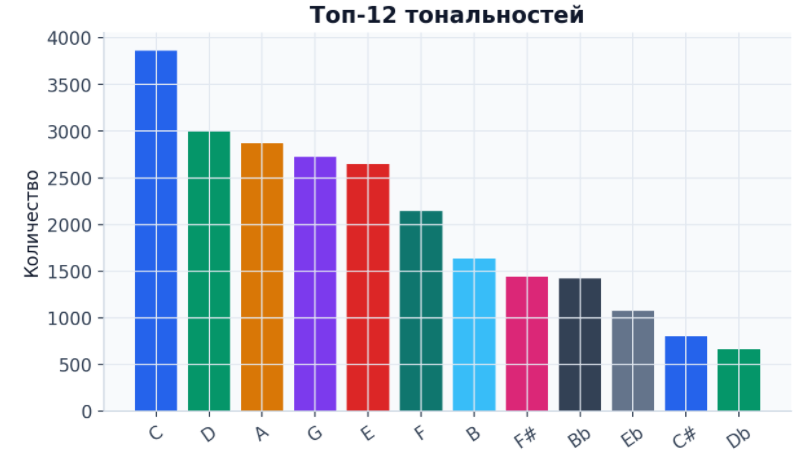
\includegraphics[width=0.94\textwidth,height=0.285\textheight,keepaspectratio]{key_distribution.png}
\captionof{figure}{Распределение тональностей внутри набора данных \textit{HookTheory Dataset}}
\label{fig:key-distribution}

\vspace{0.05\baselineskip}

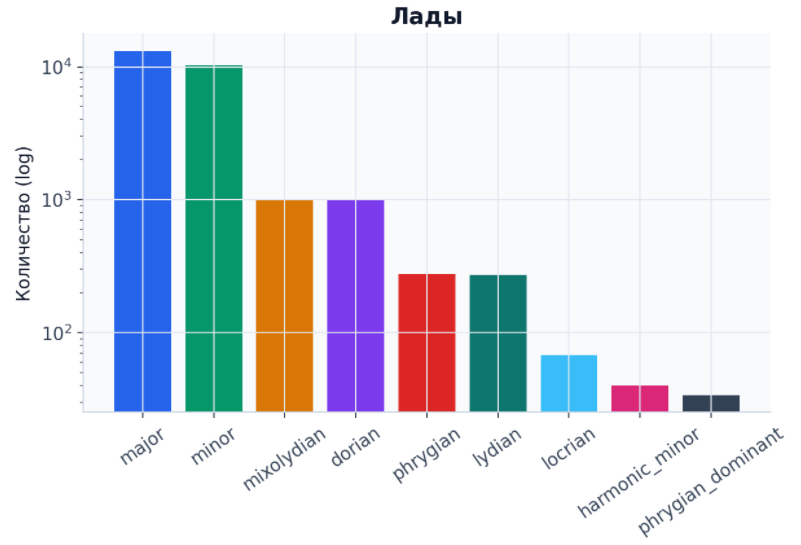
\includegraphics[width=0.94\textwidth,height=0.285\textheight,keepaspectratio]{mode_distribution.png}
\captionof{figure}{Распределение ладов внутри набора данных \textit{HookTheory Dataset}}
\label{fig:mode-distribution}

\vspace{0.05\baselineskip}

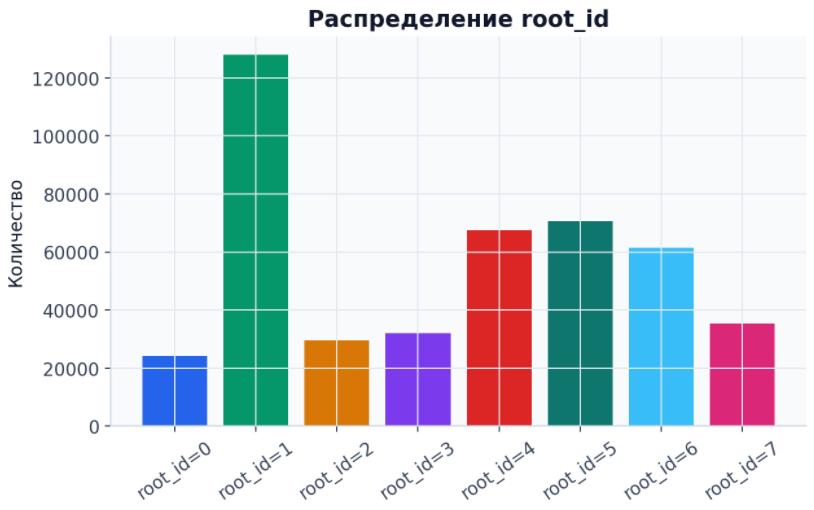
\includegraphics[width=0.94\textwidth,height=0.285\textheight,keepaspectratio]{chord_degree_distribution.png}
\captionof{figure}{Распределение ступеней аккордов внутри набора данных \textit{HookTheory Dataset}\label{fig:chord-degree-distribution}}
\end{center}

\newpage

\begin{center}
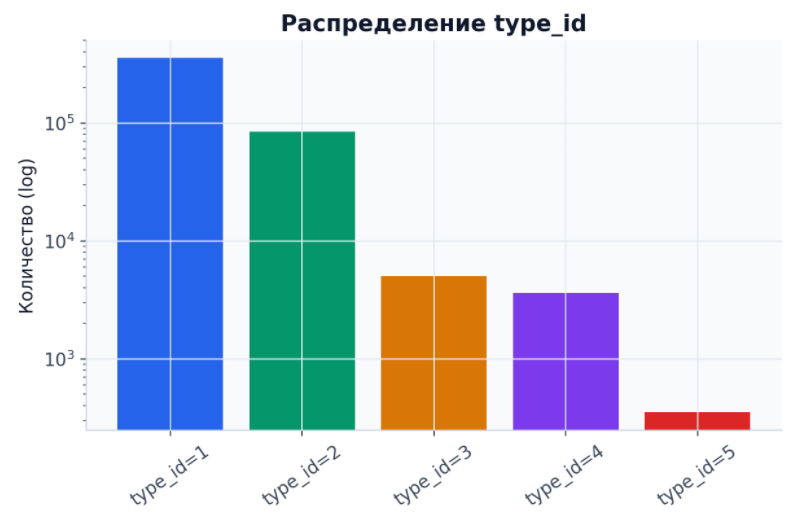
\includegraphics[width=0.94\textwidth,height=0.50\textheight,keepaspectratio]{chord_type_distribution.png}
\captionof{figure}{Распределение типов аккордов внутри набора данных \textit{HookTheory Dataset}\label{fig:chord-type-distribution}}
\end{center}

\vspace{0.25\baselineskip}

\begin{center}
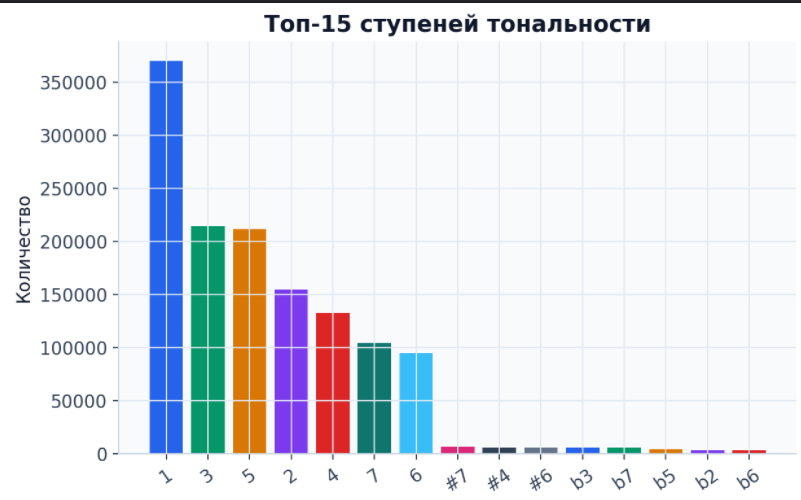
\includegraphics[width=0.9\textwidth,height=0.4\textheight,keepaspectratio]{melodic_degree_distribution.png}
\captionof{figure}{Распределение мелодических ступеней в наборе данных \textit{HookTheory Dataset}\label{fig:melodic-degree-distribution}}
\end{center}
\endgroup

\end{document}
